\part{Reinforcement Learning}

\chapter{Classical Reinforcement Learning}
\label{ch:classical-rl}

\section{Markov Decision Processes}

The foundation of reinforcement learning is the \emph{Markov Decision Process} (MDP), which formalizes sequential decision-making.

\begin{definition}[Markov Decision Process]
    An MDP is a tuple $(\mathcal{S}, \mathcal{A}, p_0, P, R, \gamma)$ where:
    \begin{itemize}
        \item $\mathcal{S}$ is the state space,
        \item $\mathcal{A}$ is the action space,
        \item $p_0(s)$ is the initial state distribution,
        \item $P(s' | s, a)$ is the transition probability (environment dynamics),
        \item $R(s, a)$ is the reward function,
        \item $\gamma \in [0,1)$ is the discount factor.
    \end{itemize}
\end{definition}

\begin{remark}[The Markov Property]
    The ``Markov'' in MDP refers to the \emph{Markov property}: the future depends only on the current state, not on how we got there:
    \[
        P(s_{t+1} | s_t, a_t, s_{t-1}, a_{t-1}, \ldots, s_0, a_0) = P(s_{t+1} | s_t, a_t).
    \]
    This means the state $s_t$ captures all relevant history. Formally, the state is a \emph{sufficient statistic} for predicting future rewards and states.

    \textbf{Why this matters:}
    \begin{itemize}
        \item Algorithms can make decisions based solely on current state---no need to track full history.
        \item Value functions $V(s)$ and $Q(s,a)$ are well-defined as functions of state alone.
        \item The Bellman equations hold, enabling dynamic programming.
    \end{itemize}

    \textbf{When does it fail?}
    In practice, the true state may be \emph{partially observable}. For example:
    \begin{itemize}
        \item A robot with limited sensors cannot observe its full position.
        \item In games, the opponent's strategy depends on history you didn't observe.
        \item In LLMs, the ``state'' (input prompt) often doesn't capture conversation context.
    \end{itemize}
    When Markov property fails, we need POMDPs (Partially Observable MDPs) or recurrent architectures that maintain memory.
\end{remark}

\begin{definition}[Policy]
    A policy $\pi: \mathcal{S} \to \Delta(\mathcal{A})$ maps states to distributions over actions. The agent's goal is to find a policy maximizing expected cumulative reward.
\end{definition}

\begin{remark}[Reward Notation]
    $R(s,a)$ is the reward \emph{function}---it takes a state-action pair and returns a number. When we write $R_t$, we mean the reward received at time $t$, i.e., $R_t = R(s_t, a_t)$.

    In classical RL, $R$ is given by the environment (e.g., +1 for winning a game). In RLHF (\cref{ch:rl-for-llms}), we don't have a true reward---instead we \emph{learn} a reward model $r_\phi(x,y)$ from human preferences. The lowercase $r$ with subscript $\phi$ emphasizes that it's a learned approximation, not ground truth.
\end{remark}

\begin{remark}[Notation]
    We write $\pi(a|s)$ for the probability of action $a$ given state $s$, and $\pi(\cdot|s)$ to denote the entire distribution over actions (the dot is a placeholder for the random variable). Thus $a \sim \pi(\cdot|s)$ means ``sample action $a$ from the distribution $\pi(\cdot|s)$.'' Similarly, $\tau \sim \pi_\theta$ means ``sample a trajectory $\tau = (s_0, a_0, s_1, a_1, \ldots)$ by rolling out the policy $\pi_\theta$.''
\end{remark}

\section{Value Functions}

Value functions quantify the expected return from states or state-action pairs.

\begin{definition}[State Value Function]
    The value function under policy $\pi$ is
    \[
        V^\pi(s) = \mathbb{E}_\pi \left[ \sum_{t=0}^{\infty} \gamma^t R(s_t, a_t) \,\Big|\, s_0 = s \right].
    \]
    The conditioning $s_0 = s$ means we average over all trajectories that start from state $s$. A trajectory $\tau = (s_0, a_0, s_1, a_1, s_2, a_2, \ldots)$ is generated by:
    \[
        a_t \sim \pi(\cdot|s_t), \quad s_{t+1} \sim P(\cdot|s_t, a_t), \quad r_t = R(s_t, a_t).
    \]
    Branching occurs due to stochasticity in both the policy and environment:
    \begin{center}
        \begin{tikzpicture}[
                state/.style={circle, draw, minimum size=0.7cm, inner sep=0pt, font=\small},
                every edge/.style={draw, ->, >=stealth}
            ]
            % Main trajectory (highlighted)
            \node[state, fill=blue!20] (s0) {$s_0$};
            \node[state] (s1) at ($(s0) + (2.2, 0)$) {$s_1$};
            \node[state] (s2) at ($(s1) + (2.2, 0)$) {$s_2$};
            \node (dots) at ($(s2) + (1.5, 0)$) {$\cdots$};

            % Edges with action labels
            \draw[->] (s0) -- node[above, font=\footnotesize] {$a_0$} node[below, font=\footnotesize, color=green!50!black] {$r_0$} (s1);
            \draw[->] (s1) -- node[above, font=\footnotesize] {$a_1$} node[below, font=\footnotesize, color=green!50!black] {$r_1$} (s2);
            \draw[->] (s2) -- node[above, font=\footnotesize] {$a_2$} node[below, font=\footnotesize, color=green!50!black] {$r_2$} (dots);

            % Alternative branches from s0 (showing stochasticity)
            \node[state, color=gray] (s1a) at ($(s0) + (1.8, -1.2)$) {};
            \node[state, color=gray] (s1b) at ($(s0) + (2.0, 1.0)$) {};
            \draw[->, gray, dashed] (s0) -- node[below left, font=\tiny, color=gray] {$a'_0$} (s1a);
            \draw[->, gray, dashed] (s0) -- node[above left, font=\tiny, color=gray] {$a''_0$} (s1b);

            % Alternative branches from s1
            \node[state, color=gray] (s2a) at ($(s1) + (1.8, -1.0)$) {};
            \draw[->, gray, dashed] (s1) -- (s2a);

            % Annotations
            \node[anchor=west, font=\footnotesize] at ($(dots) + (0.5, 0)$) {$G = r_0 + \gamma r_1 + \gamma^2 r_2 + \cdots$};
            \node[anchor=north, font=\footnotesize, color=gray] at ($(s1a) + (0, -0.3)$) {other samples};
        \end{tikzpicture}
    \end{center}
    Sampling $N$ trajectories from $s$ and averaging their returns gives:
    \begin{center}
        \begin{tikzpicture}[
                state/.style={circle, draw, minimum size=0.5cm, inner sep=0pt, font=\tiny},
                traj/.style={thick}
            ]
            \node[state, fill=blue!20] (s) {$s$};

            % Trajectory 1
            \node[state] (s11) at ($(s) + (-2.2, -1.0)$) {};
            \node[state] (s12) at ($(s11) + (-0.4, -0.8)$) {};
            \node[font=\small] (g1) at ($(s12) + (0, -0.6)$) {$G^{(1)}$};

            % Trajectory 2
            \node[state] (s21) at ($(s) + (-0.7, -1.0)$) {};
            \node[state] (s22) at ($(s21) + (0.2, -0.8)$) {};
            \node[font=\small] (g2) at ($(s22) + (0, -0.6)$) {$G^{(2)}$};

            % Trajectory 3
            \node[state] (s31) at ($(s) + (0.7, -1.0)$) {};
            \node[state] (s32) at ($(s31) + (-0.1, -0.8)$) {};
            \node[font=\small] (g3) at ($(s32) + (0, -0.6)$) {$G^{(3)}$};

            % Trajectory N
            \node[state] (sn1) at ($(s) + (2.2, -1.0)$) {};
            \node[state] (sn2) at ($(sn1) + (0.3, -0.8)$) {};
            \node[font=\small] (gn) at ($(sn2) + (0, -0.6)$) {$G^{(N)}$};

            % Dots
            \node at ($(s) + (1.5, -1.0)$) {$\cdots$};

            % Edges
            \draw[->] (s) -- (s11); \draw[->] (s11) -- (s12); \draw[->, dashed] (s12) -- (g1);
            \draw[->] (s) -- (s21); \draw[->] (s21) -- (s22); \draw[->, dashed] (s22) -- (g2);
            \draw[->] (s) -- (s31); \draw[->] (s31) -- (s32); \draw[->, dashed] (s32) -- (g3);
            \draw[->] (s) -- (sn1); \draw[->] (sn1) -- (sn2); \draw[->, dashed] (sn2) -- (gn);

            % Formula
            \node[font=\small] at (0, -3.8) {$V^\pi(s) \approx \frac{1}{N}\bigl(G^{(1)} + G^{(2)} + \cdots + G^{(N)}\bigr)$};
        \end{tikzpicture}
    \end{center}
    In practice, this expectation is estimated via Monte Carlo sampling:
    \[
        V^\pi(s) \approx \frac{1}{N} \sum_{i=1}^{N} G^{(i)}, \quad \text{where } G^{(i)} = \sum_{t=0}^{T} \gamma^t R(s_t^{(i)}, a_t^{(i)})
    \]
    and each trajectory $\tau^{(i)} = (s, a_0^{(i)}, s_1^{(i)}, \ldots)$ is sampled by starting from $s$ and following $\pi$.
\end{definition}

\begin{definition}[Action-Value Function]
    The Q-function under policy $\pi$ is
    \[
        Q^\pi(s, a) = \mathbb{E}_\pi \left[ \sum_{t=0}^{\infty} \gamma^t R(s_t, a_t) \,\Big|\, s_0 = s, a_0 = a \right].
    \]
    Here the conditioning $s_0 = s, a_0 = a$ means we fix the initial state-action pair and average over all continuations under $\pi$.
\end{definition}

The relationship between them:
\[
    V^\pi(s) = \mathbb{E}_{a \sim \pi(\cdot|s)}[Q^\pi(s,a)] = \sum_{a} \pi(a|s) Q^\pi(s,a).
\]

\begin{definition}[Advantage Function]
    The advantage function measures how much better an action is compared to the average:
    \[
        A^\pi(s, a) = Q^\pi(s, a) - V^\pi(s).
    \]
\end{definition}

\section{Bellman Equations}

The Bellman equations transform an intractable problem (optimize over infinite trajectories) into a tractable one (solve a system of equations). They are the foundation of nearly all RL algorithms.

\subsection{The Equations}

\begin{proposition}[Bellman Expectation Equation]
    The value function satisfies the recursive relation:
    \[
        V^\pi(s) = \sum_{a} \pi(a|s) \left[ R(s,a) + \gamma \sum_{s'} P(s'|s,a) V^\pi(s') \right].
    \]
\end{proposition}

\begin{proof}
    Start from the definition and split the first step from the rest:
    \begin{align*}
        V^\pi(s) & = \mathbb{E}_\pi\left[ \sum_{t=0}^{\infty} \gamma^t R_t \,\Big|\, s_0 = s \right]                                                                                                                    \\
                 & = \mathbb{E}_\pi\left[ R_0 + \sum_{t=1}^{\infty} \gamma^t R_t \,\Big|\, s_0 = s \right]                                                                                                              \\
                 & = \mathbb{E}_\pi\left[ R_0 + \gamma \sum_{t=0}^{\infty} \gamma^t R_{t+1} \,\Big|\, s_0 = s \right]                                                                                                   \\
                 & = \mathbb{E}_{a \sim \pi(\cdot|s)}\left[ R(s,a) + \gamma \, \mathbb{E}_{s' \sim P(\cdot|s,a)}\left[ \mathbb{E}_\pi\left[ \sum_{t=0}^{\infty} \gamma^t R_t \,\Big|\, s_0 = s' \right] \right] \right]
    \end{align*}
    The inner expectation is exactly $V^\pi(s')$ by the Markov property. Writing out the expectations as sums:
    \[
        V^\pi(s) = \sum_{a} \pi(a|s) \left[ R(s,a) + \gamma \sum_{s'} P(s'|s,a) V^\pi(s') \right]. \qedhere
    \]
\end{proof}

\begin{remark}[Intuition]
    The Bellman equation says: the value of state $s$ equals the immediate reward plus the discounted value of where we end up. This recursive structure is what enables dynamic programming algorithms (value iteration, policy iteration).
\end{remark}

\begin{proposition}[Bellman Optimality Equation]
    The optimal value function $V^* = \max_\pi V^\pi$ satisfies:
    \[
        V^*(s) = \max_{a} \left[ R(s,a) + \gamma \sum_{s'} P(s'|s,a) V^*(s') \right].
    \]
    Similarly for the optimal Q-function:
    \[
        Q^*(s,a) = R(s,a) + \gamma \sum_{s'} P(s'|s,a) \max_{a'} Q^*(s', a').
    \]
\end{proposition}

\begin{proof}
    The optimal policy at state $s$ must choose the action that maximizes expected return. Suppose we act optimally from $s$ onwards:
    \begin{align*}
        V^*(s) & = \max_\pi V^\pi(s)                                                  \\
               & = \max_a \left[ R(s,a) + \gamma \sum_{s'} P(s'|s,a) V^*(s') \right].
    \end{align*}
    The $\max$ over policies reduces to $\max$ over the first action because, by the principle of optimality, whatever action we take now, we should act optimally thereafter---and $V^*(s')$ already captures optimal future behavior.

    For $Q^*$: if we take action $a$ in state $s$ and then act optimally:
    \[
        Q^*(s,a) = R(s,a) + \gamma \sum_{s'} P(s'|s,a) V^*(s') = R(s,a) + \gamma \sum_{s'} P(s'|s,a) \max_{a'} Q^*(s', a'). \qedhere
    \]
\end{proof}

\subsection{Why Bellman Equations Matter}

\begin{remark}[From Definition to Algorithm]
    Without Bellman equations, computing $V^\pi(s)$ requires:
    \[
        V^\pi(s) = \mathbb{E}\left[ \sum_{t=0}^{\infty} \gamma^t R_t \,\Big|\, s_0 = s \right] \quad \text{--- average over infinitely many infinite trajectories.}
    \]
    The Bellman equation converts this into a \emph{system of $|\mathcal{S}|$ linear equations}:
    \[
        V^\pi(s) = \sum_{a} \pi(a|s) \left[ R(s,a) + \gamma \sum_{s'} P(s'|s,a) V^\pi(s') \right] \quad \text{for each } s \in \mathcal{S}.
    \]
    This can be solved exactly (matrix inversion) or iteratively.
\end{remark}

\begin{definition}[Value Iteration]
    To find the optimal value function $V^*$, repeatedly apply the Bellman optimality operator:
    \[
        V_{k+1}(s) \leftarrow \max_{a} \left[ R(s,a) + \gamma \sum_{s'} P(s'|s,a) V_k(s') \right] \quad \text{for all } s.
    \]
    Start with arbitrary $V_0$. As $k \to \infty$, $V_k \to V^*$.
\end{definition}

\begin{remark}[Why It Converges]
    The Bellman operator is a \emph{contraction} with factor $\gamma < 1$. By the Banach fixed-point theorem, repeated application converges to the unique fixed point $V^*$.
\end{remark}

\begin{definition}[Q-Learning Update]
    When the environment dynamics $P(s'|s,a)$ are unknown, we learn $Q^*$ from experience. After observing transition $(s, a, r, s')$:
    \[
        Q(s,a) \leftarrow Q(s,a) + \alpha \left[ \underbrace{r + \gamma \max_{a'} Q(s', a')}_{\text{Bellman target}} - Q(s,a) \right].
    \]
    This is a stochastic approximation of value iteration, using samples instead of the full expectation.
\end{definition}

\begin{remark}[The Bellman Equation in Disguise]
    Q-learning works because it's trying to satisfy:
    \[
        Q^*(s,a) = \mathbb{E}\left[ r + \gamma \max_{a'} Q^*(s',a') \right].
    \]
    Each update nudges $Q(s,a)$ toward the right-hand side. At convergence, the Bellman equation holds.
\end{remark}

\begin{remark}[Connection to Policy Gradient]
    Even policy gradient methods use Bellman ideas:
    \begin{itemize}
        \item The \textbf{advantage} $A^\pi(s,a) = Q^\pi(s,a) - V^\pi(s)$ requires estimating $V^\pi$ or $Q^\pi$.
        \item \textbf{Actor-critic} methods learn $V^\pi$ (the critic) using Bellman updates, then use it to compute advantages for policy gradient (the actor).
        \item \textbf{GAE} (Generalized Advantage Estimation) uses the Bellman structure: $\delta_t = r_t + \gamma V(s_{t+1}) - V(s_t)$ is the \emph{TD error}, measuring how wrong the current $V$ is.
    \end{itemize}
    The Bellman equation is not an alternative to policy gradient---it's a tool used \emph{within} policy gradient methods.
\end{remark}

\section{Temporal Difference Learning}

TD learning bridges Monte Carlo methods (which wait for complete episodes) and dynamic programming (which requires a model).

\begin{definition}[TD(0) Update]
    After observing transition $(s_t, a_t, r_t, s_{t+1})$, update the value function:
    \[
        V(s_t) \leftarrow V(s_t) + \alpha \underbrace{\bigl[ r_t + \gamma V(s_{t+1}) - V(s_t) \bigr]}_{\delta_t \text{ (TD error)}}.
    \]
    The TD error $\delta_t$ measures how ``surprised'' we are: if $r_t + \gamma V(s_{t+1}) > V(s_t)$, the outcome was better than expected.
\end{definition}

\begin{center}
    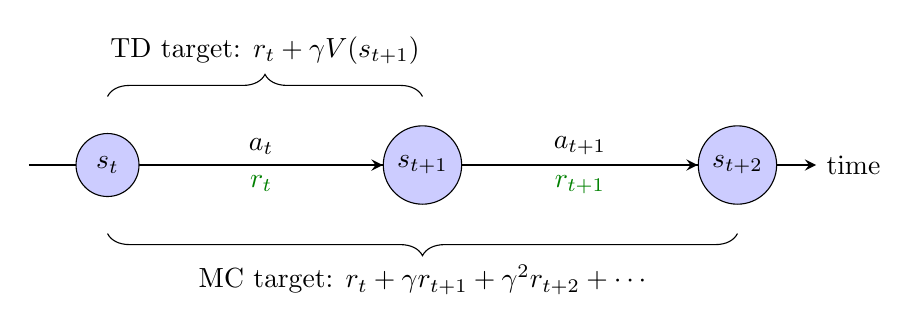
\begin{tikzpicture}[>=stealth]
        % Timeline
        \draw[thick, ->] (0,0) -- (10,0) node[right] {time};

        % States
        \node[circle, draw, fill=blue!20, minimum size=8mm] (s0) at (1,0) {$s_t$};
        \node[circle, draw, fill=blue!20, minimum size=8mm] (s1) at (5,0) {$s_{t+1}$};
        \node[circle, draw, fill=blue!20, minimum size=8mm] (s2) at (9,0) {$s_{t+2}$};

        % Arrows with rewards
        \draw[->, thick] (s0) -- node[above] {$a_t$} node[below, green!50!black] {$r_t$} (s1);
        \draw[->, thick] (s1) -- node[above] {$a_{t+1}$} node[below, green!50!black] {$r_{t+1}$} (s2);

        % TD target annotation
        \draw[decorate, decoration={brace, amplitude=8pt, raise=2pt}] (1,0.8) -- (5,0.8)
        node[midway, above=10pt] {TD target: $r_t + \gamma V(s_{t+1})$};

        % Monte Carlo annotation
        \draw[decorate, decoration={brace, amplitude=8pt, raise=2pt, mirror}] (1,-0.8) -- (9,-0.8)
        node[midway, below=10pt] {MC target: $r_t + \gamma r_{t+1} + \gamma^2 r_{t+2} + \cdots$};
    \end{tikzpicture}
\end{center}

\begin{remark}[TD vs Monte Carlo]
    \begin{center}
        \begin{tabular}{l|cc}
                     & \textbf{Monte Carlo}                         & \textbf{TD(0)}             \\
            \hline
            Updates  & End of episode                               & Every step                 \\
            Target   & $G_t = \sum_{k=0}^{\infty} \gamma^k r_{t+k}$ & $r_t + \gamma V(s_{t+1})$  \\
            Bias     & Unbiased                                     & Biased (uses estimate $V$) \\
            Variance & High                                         & Lower                      \\
            Requires & Complete episodes                            & Only $(s,a,r,s')$ tuples   \\
        \end{tabular}
    \end{center}
    TD methods \emph{bootstrap}---they update estimates based on other estimates. This introduces bias but dramatically reduces variance.
\end{remark}

\begin{definition}[TD($\lambda$) and Eligibility Traces]
    TD($\lambda$) interpolates between TD(0) ($\lambda=0$) and Monte Carlo ($\lambda=1$):
    \[
        G_t^\lambda = (1-\lambda) \sum_{n=1}^{\infty} \lambda^{n-1} G_t^{(n)}
    \]
    where $G_t^{(n)} = r_t + \gamma r_{t+1} + \cdots + \gamma^{n-1} r_{t+n-1} + \gamma^n V(s_{t+n})$ is the $n$-step return.

    Equivalently, using \emph{eligibility traces}:
    \[
        e_t(s) = \gamma \lambda e_{t-1}(s) + \mathbf{1}[s_t = s], \quad V(s) \leftarrow V(s) + \alpha \delta_t e_t(s).
    \]
\end{definition}

\begin{center}
    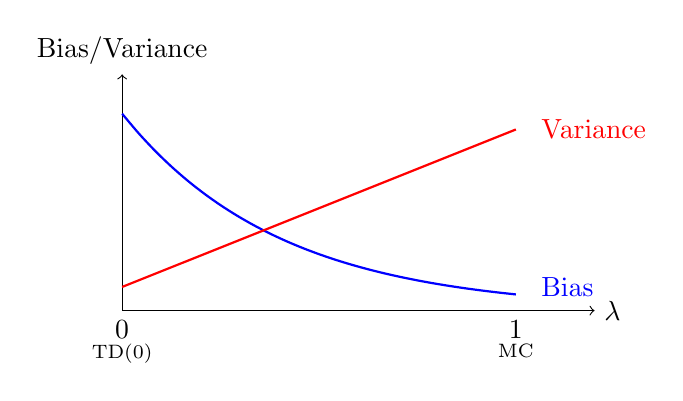
\begin{tikzpicture}
        \draw[->] (0,0) -- (6,0) node[right] {$\lambda$};
        \draw[->] (0,0) -- (0,3) node[above] {Bias/Variance};

        % Bias curve (decreasing)
        \draw[thick, blue] plot[smooth, domain=0:5] (\x, {2.5*exp(-0.5*\x)});
        \node[blue, right] at (5.2, 0.3) {Bias};

        % Variance curve (increasing)
        \draw[thick, red] plot[smooth, domain=0:5] (\x, {0.3 + 0.4*\x});
        \node[red, right] at (5.2, 2.3) {Variance};

        % Labels
        \node[below] at (0,0) {$0$};
        \node[below] at (5,0) {$1$};
        \node[below] at (0,-0.3) {\scriptsize TD(0)};
        \node[below] at (5,-0.3) {\scriptsize MC};
    \end{tikzpicture}
\end{center}

\section{Policy Gradient Methods}

When the policy is parameterized by $\theta$, we directly optimize the expected return.

\subsection{Why This Objective?}

The goal is to find a policy that maximizes total reward over time. But which total?

\begin{itemize}
    \item \textbf{Finite horizon}: $\sum_{t=0}^{T} R_t$ — sum rewards for $T$ steps. Simple, but what is $T$?
    \item \textbf{Infinite horizon (undiscounted)}: $\sum_{t=0}^{\infty} R_t$ — can diverge to $\infty$.
    \item \textbf{Infinite horizon (discounted)}: $\sum_{t=0}^{\infty} \gamma^t R_t$ — always finite if rewards are bounded.
\end{itemize}

The discounted sum $\sum_{t=0}^{\infty} \gamma^t R_t$ with $\gamma \in [0,1)$ is the standard choice:
\begin{center}
    \begin{tikzpicture}
        \draw[->] (0,0) -- (8,0) node[right] {$t$};
        \draw[->] (0,0) -- (0,2.5) node[above] {$\gamma^t$};

        % Gamma curve
        \draw[thick, blue] plot[domain=0:7, samples=50] (\x, {2*0.8^\x});

        % Points with labels
        \foreach \t in {0,1,2,3,4,5,6} {
                \fill[blue] (\t, {2*0.8^\t}) circle (2pt);
            }

        % x-axis labels
        \node[below] at (0,0) {$0$};
        \node[below] at (1,0) {$1$};
        \node[below] at (2,0) {$2$};
        \node[below] at (3,0) {$3$};

        % Only label 1 on y-axis
        \node[left] at (0,2) {$1$};

        \node[anchor=west] at (5, 1.5) {$\gamma = 0.8$};
    \end{tikzpicture}
\end{center}

\begin{remark}[Why Discount?]
    The discount factor $\gamma < 1$ serves multiple purposes:
    \begin{enumerate}
        \item \textbf{Convergence}: Ensures $\sum_{t=0}^{\infty} \gamma^t R_t < \infty$ even for infinite horizons.
        \item \textbf{Preference for sooner rewards}: Reward now is worth more than reward later (like money).
        \item \textbf{Uncertainty}: The further into the future, the less certain our predictions.
        \item \textbf{Effective horizon}: Most of the weight is on the first $\approx \frac{1}{1-\gamma}$ steps.
              For $\gamma = 0.99$, this is $\approx 100$ steps; for $\gamma = 0.9$, only $\approx 10$ steps.
    \end{enumerate}
\end{remark}

\begin{remark}[Trajectory Structure]
    A trajectory $\tau = (s_0, a_0, s_1, a_1, \ldots)$ is generated by alternating between policy and environment:
    \begin{enumerate}
        \item \textbf{Agent chooses action}: Given $s_t$, policy outputs $a_t$ with probability $\pi_\theta(a_t|s_t)$.
        \item \textbf{Environment transitions}: Given $(s_t, a_t)$, next state is $s_{t+1}$ with probability $P(s_{t+1}|s_t,a_t)$.
    \end{enumerate}
    \begin{center}
        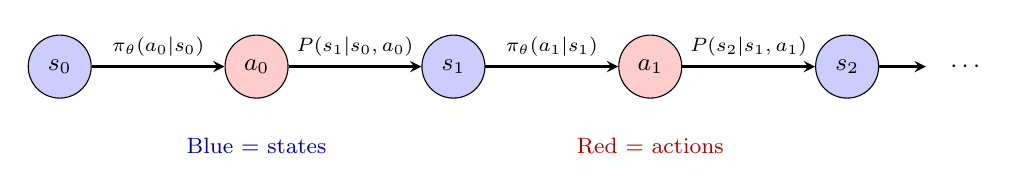
\begin{tikzpicture}[>=stealth, every node/.style={font=\small}]
            \node[circle, draw, fill=blue!20, minimum size=8mm] (s0) at (0,0) {$s_0$};
            \node[circle, draw, fill=red!20, minimum size=8mm] (a0) at (2.5,0) {$a_0$};
            \node[circle, draw, fill=blue!20, minimum size=8mm] (s1) at (5,0) {$s_1$};
            \node[circle, draw, fill=red!20, minimum size=8mm] (a1) at (7.5,0) {$a_1$};
            \node[circle, draw, fill=blue!20, minimum size=8mm] (s2) at (10,0) {$s_2$};
            \node at (11.5,0) {$\cdots$};

            \draw[->, thick] (s0) -- node[above, font=\scriptsize] {$\pi_\theta(a_0|s_0)$} (a0);
            \draw[->, thick] (a0) -- node[above, font=\scriptsize] {$P(s_1|s_0,a_0)$} (s1);
            \draw[->, thick] (s1) -- node[above, font=\scriptsize] {$\pi_\theta(a_1|s_1)$} (a1);
            \draw[->, thick] (a1) -- node[above, font=\scriptsize] {$P(s_2|s_1,a_1)$} (s2);
            \draw[->, thick] (s2) -- (11,0);

            \node[blue!70!black, font=\footnotesize] at (2.5, -1) {Blue = states};
            \node[red!70!black, font=\footnotesize] at (7.5, -1) {Red = actions};
        \end{tikzpicture}
    \end{center}
\end{remark}

\begin{example}[Classic RL --- Robot on Slippery Floor]
    State $s$ = robot position. Action $a$ = movement command. The robot is at $(2,3)$ and commands ``right'':
    \begin{center}
        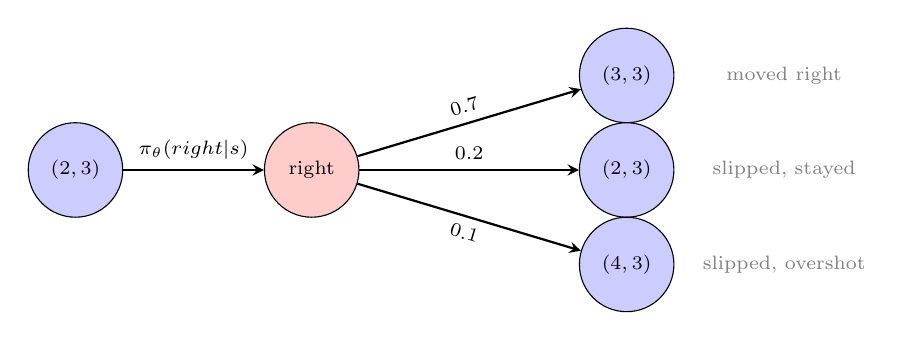
\begin{tikzpicture}[>=stealth, every node/.style={font=\small}]
            \node[circle, draw, fill=blue!20, minimum size=12mm] (s0) at (0,0) {\scriptsize $(2,3)$};
            \node[circle, draw, fill=red!20, minimum size=12mm] (a0) at (3,0) {\scriptsize right};

            % Multiple possible outcomes
            \node[circle, draw, fill=blue!20, minimum size=12mm] (s1a) at (7,1.2) {\scriptsize $(3,3)$};
            \node[circle, draw, fill=blue!20, minimum size=12mm] (s1b) at (7,0) {\scriptsize $(2,3)$};
            \node[circle, draw, fill=blue!20, minimum size=12mm] (s1c) at (7,-1.2) {\scriptsize $(4,3)$};

            \draw[->, thick] (s0) -- node[above, font=\scriptsize] {$\pi_\theta(\text{right}|s)$} (a0);
            \draw[->, thick] (a0) -- node[above, font=\scriptsize, sloped] {$0.7$} (s1a);
            \draw[->, thick] (a0) -- node[above, font=\scriptsize] {$0.2$} (s1b);
            \draw[->, thick] (a0) -- node[below, font=\scriptsize, sloped] {$0.1$} (s1c);

            % Labels
            \node[font=\scriptsize, gray] at (9, 1.2) {moved right};
            \node[font=\scriptsize, gray] at (9, 0) {slipped, stayed};
            \node[font=\scriptsize, gray] at (9, -1.2) {slipped, overshot};
        \end{tikzpicture}
    \end{center}
    The transition probabilities $P(s'|s,a)$ form a distribution over next states:
    \[
        P\bigl((3,3) \,\big|\, (2,3), \text{right}\bigr) = 0.7, \quad
        P\bigl((2,3) \,\big|\, (2,3), \text{right}\bigr) = 0.2, \quad
        P\bigl((4,3) \,\big|\, (2,3), \text{right}\bigr) = 0.1.
    \]
    The agent chose ``right'', but \emph{physics decides where it actually lands}. This environment randomness is outside the agent's control.
\end{example}

\begin{example}[LLM Text Generation]
    State $s$ = tokens so far. Action $a$ = next token. The LLM has generated ``The cat'' and samples ``sat'':
    \begin{center}
        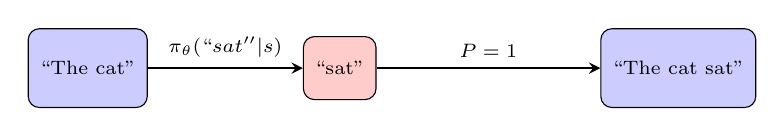
\begin{tikzpicture}[>=stealth, every node/.style={font=\small}]
            \node[rounded corners, draw, fill=blue!20, minimum height=10mm, inner sep=4pt] (s0) at (0,0) {\scriptsize ``The cat''};
            \node[rounded corners, draw, fill=red!20, minimum height=8mm, inner sep=4pt] (a0) at (3.2,0) {\scriptsize ``sat''};
            \node[rounded corners, draw, fill=blue!20, minimum height=10mm, inner sep=4pt] (s1) at (7.5,0) {\scriptsize ``The cat sat''};

            \draw[->, thick] (s0) -- node[above, font=\scriptsize] {$\pi_\theta(\text{``sat''}|s)$} (a0);
            \draw[->, thick] (a0) -- node[above, font=\scriptsize] {$P=1$} (s1);
        \end{tikzpicture}
    \end{center}
    There is only \emph{one possible next state}: the concatenation. The transition is deterministic:
    \[
        P\bigl(\text{``The cat sat''} \,\big|\, \text{``The cat''}, \text{``sat''}\bigr) = 1.
    \]
    All other next states have probability 0. The ``environment'' is just string concatenation---it contributes \emph{zero randomness}.
\end{example}

\begin{remark}[Where Does Randomness Live?]
    This distinction is fundamental:
    \begin{center}
        \begin{tabular}{l|cc}
                  & \textbf{Policy} $\pi_\theta(a|s)$ & \textbf{Environment} $P(s'|s,a)$ \\
            \hline
            Robot & stochastic                        & stochastic                       \\
            LLM   & stochastic                        & deterministic ($P=1$)
        \end{tabular}
    \end{center}
    In LLMs, \emph{all trajectory randomness comes from the policy}. This is why LLM fine-tuning (RLHF, DPO, etc.) focuses entirely on modifying $\pi_\theta$---there is no environment to model or fight against.
\end{remark}

\begin{definition}[RL Objective]
    The objective is the expected discounted return:
    \[
        J(\theta) = \mathbb{E}_{\tau \sim \pi_\theta} \left[ \sum_{t=0}^{\infty} \gamma^t R(s_t, a_t) \right]
    \]
    where $\tau = (s_0, a_0, s_1, a_1, \ldots)$ is a trajectory sampled by following policy $\pi_\theta$.
\end{definition}

\begin{theorem}[Policy Gradient Theorem]
    The gradient of the objective is
    \[
        \nabla_\theta J(\theta) = \mathbb{E}_{\tau \sim \pi_\theta} \left[ \sum_{t=0}^{\infty} \nabla_\theta \log \pi_\theta(a_t | s_t) \cdot G_t \right]
    \]
    where $G_t = \sum_{k=t}^{\infty} \gamma^{k-t} R(s_k, a_k)$ is the return from time $t$.
\end{theorem}

\begin{proof}
    Starting from $J(\theta) = \mathbb{E}_{\tau}[R(\tau)]$:
    \begin{align*}
        \nabla_\theta J(\theta) & = \nabla_\theta \int p_\theta(\tau) R(\tau) \, d\tau                                          \\
                                & = \int R(\tau) \nabla_\theta p_\theta(\tau) \, d\tau                                          \\
                                & = \int R(\tau) p_\theta(\tau) \nabla_\theta \log p_\theta(\tau) \, d\tau                      \\
                                & = \mathbb{E}_{\tau \sim \pi_\theta} \left[ R(\tau) \nabla_\theta \log p_\theta(\tau) \right].
    \end{align*}
    For the trajectory probability, by chain rule:
    \[
        p_\theta(\tau) = p_0(s_0) \prod_{t=0}^{\infty} \pi_\theta(a_t|s_t) \cdot P(s_{t+1}|s_t,a_t).
    \]
    Taking logs:
    \[
        \log p_\theta(\tau) = \underbrace{\log p_0(s_0)}_{\text{no } \theta} + \sum_t \underbrace{\log \pi_\theta(a_t|s_t)}_{\text{depends on } \theta} + \sum_t \underbrace{\log P(s_{t+1}|s_t,a_t)}_{\text{no } \theta}.
    \]
    Only $\pi_\theta$ terms depend on $\theta$, so $\nabla_\theta \log p_\theta(\tau) = \sum_{t} \nabla_\theta \log \pi_\theta(a_t | s_t)$.

    Substituting with $R(\tau) = \sum_{t=0}^{\infty} \gamma^t R_t$:
    \[
        \nabla_\theta J = \mathbb{E}\left[ \left(\sum_{t'} \gamma^{t'} R_{t'}\right) \left(\sum_t \nabla_\theta \log \pi_\theta(a_t|s_t)\right) \right].
    \]

    \textbf{The Causality Argument:} Consider the cross terms $R_{t'} \cdot \nabla_\theta \log \pi_\theta(a_t|s_t)$ for $t' < t$:
    \begin{itemize}
        \item $R_{t'}$ depends only on $(s_{t'}, a_{t'})$, which are determined \emph{before} action $a_t$ is chosen.
        \item $\nabla_\theta \log \pi_\theta(a_t|s_t)$ depends on action $a_t$.
        \item Since $a_t \sim \pi_\theta(\cdot|s_t)$ is sampled \emph{independently} of the past reward $R_{t'}$ (given $s_t$):
    \end{itemize}
    \[
        \mathbb{E}\bigl[R_{t'} \cdot \nabla_\theta \log \pi_\theta(a_t|s_t)\bigr] = \mathbb{E}[R_{t'}] \cdot \underbrace{\mathbb{E}_{a_t}\bigl[\nabla_\theta \log \pi_\theta(a_t|s_t)\bigr]}_{= 0}.
    \]
    The second factor is zero because $\mathbb{E}_{a \sim \pi}[\nabla \log \pi(a)] = \sum_a \pi(a) \frac{\nabla \pi(a)}{\pi(a)} = \nabla \sum_a \pi(a) = \nabla 1 = 0$.

    Thus, only $t' \geq t$ terms contribute. Rearranging:
    \[
        \nabla_\theta J = \mathbb{E}\left[ \sum_t \nabla_\theta \log \pi_\theta(a_t|s_t) \cdot \underbrace{\sum_{t' \geq t} \gamma^{t'} R_{t'}}_{= \gamma^t G_t} \right] = \mathbb{E}\left[ \sum_t \gamma^t \nabla_\theta \log \pi_\theta(a_t|s_t) \cdot G_t \right].
    \]
    (The $\gamma^t$ can be absorbed into how we weight time steps, giving the stated form.) \qedhere
\end{proof}

\begin{remark}[Intuition for Causality]
    The action at time $t$ cannot influence rewards that already happened ($t' < t$). Including past rewards in the gradient estimate only adds noise---they're independent of the action we're evaluating. By using $G_t$ (future returns only), we reduce variance without introducing bias.

    \begin{center}
        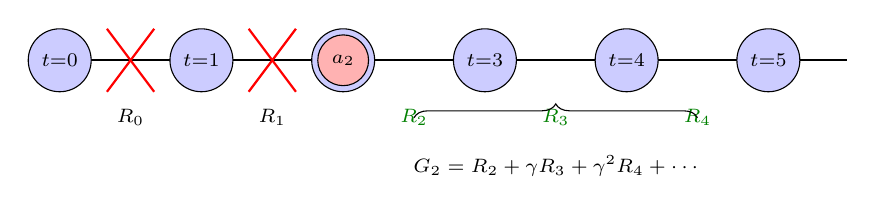
\begin{tikzpicture}[>=stealth]
            \draw[thick] (0,0) -- (10,0);
            \foreach \t in {0,1,2,3,4,5} {
                    \node[circle, draw, fill=blue!20, minimum size=5mm, font=\scriptsize] (s\t) at (1.8*\t, 0) {$t{=}\t$};
                }

            % Highlight action at t=2
            \node[circle, draw, fill=red!30, minimum size=5mm, font=\scriptsize] at (3.6, 0) {$a_2$};

            % Past rewards (crossed out)
            \draw[thick, red] (0.6, 0.4) -- (1.2, -0.4);
            \draw[thick, red] (0.6, -0.4) -- (1.2, 0.4);
            \node[below, font=\scriptsize] at (0.9, -0.5) {$R_0$};

            \draw[thick, red] (2.4, 0.4) -- (3.0, -0.4);
            \draw[thick, red] (2.4, -0.4) -- (3.0, 0.4);
            \node[below, font=\scriptsize] at (2.7, -0.5) {$R_1$};

            % Future rewards (included)
            \node[below, font=\scriptsize, green!50!black] at (4.5, -0.5) {$R_2$};
            \node[below, font=\scriptsize, green!50!black] at (6.3, -0.5) {$R_3$};
            \node[below, font=\scriptsize, green!50!black] at (8.1, -0.5) {$R_4$};

            % Annotation
            \draw[decorate, decoration={brace, amplitude=5pt, raise=2pt}] (4.5, -0.8) -- (8.1, -0.8)
            node[midway, below=8pt, font=\scriptsize] {$G_2 = R_2 + \gamma R_3 + \gamma^2 R_4 + \cdots$};
        \end{tikzpicture}
    \end{center}
\end{remark}

\begin{definition}[Policy Gradient Methods]
    A \emph{policy gradient} algorithm directly maximizes $J(\theta)$ by stochastic gradient ascent on the parameters of a differentiable policy $\pi_\theta$.
    The vanilla update is
    \[
        \theta_{k+1} = \theta_k + \alpha \, \mathbb{E}_t \bigl[ \nabla_\theta \log \pi_\theta(a_t|s_t) \, \widehat{A}_t \bigr],
    \]
    where $\widehat{A}_t$ is an estimator of the advantage $A^\pi(s_t, a_t)$ (often the Monte Carlo return minus a baseline).
    All later variants (e.g., TRPO, PPO) modify this basic gradient ascent step to control variance and stabilize updates.
\end{definition}

\begin{remark}[Variance Reduction via Baselines]
    The policy gradient theorem gives us:
    \[
        \nabla_\theta J(\theta) = \mathbb{E}_{\tau \sim \pi_\theta} \left[ \sum_{t} \nabla_\theta \log \pi_\theta(a_t | s_t) \cdot G_t \right]
    \]
    where $G_t = \sum_{k=t}^{\infty} \gamma^{k-t} R_k$ is the return from time $t$. We can subtract any \emph{baseline} $b(s_t)$ that depends only on the state:
    \[
        \nabla_\theta J(\theta) = \mathbb{E} \left[ \sum_{t} \nabla_\theta \log \pi_\theta(a_t | s_t) \cdot \bigl(G_t - b(s_t)\bigr) \right].
    \]
    This doesn't change the expectation because:
    \[
        \mathbb{E}_{a_t \sim \pi_\theta(\cdot|s_t)}\bigl[\nabla_\theta \log \pi_\theta(a_t|s_t) \cdot b(s_t)\bigr] = b(s_t) \cdot \underbrace{\sum_{a} \nabla_\theta \pi_\theta(a|s_t)}_{= \nabla_\theta 1 = 0} = 0.
    \]
    The optimal baseline (minimizing variance) is $b(s_t) = V^\pi(s_t)$. With this choice, $G_t - V^\pi(s_t)$ is an estimate of the advantage $A^\pi(s_t, a_t) = Q^\pi(s_t, a_t) - V^\pi(s_t)$.
\end{remark}

\subsection{Actor-Critic Methods}

The Actor-Critic architecture combines policy gradient (actor) with value function learning (critic).

\begin{definition}[Actor-Critic]
    An \emph{actor-critic} algorithm maintains two components:
    \begin{itemize}
        \item \textbf{Actor} $\pi_\theta(a|s)$: the policy, updated via policy gradient.
        \item \textbf{Critic} $V_\phi(s)$ or $Q_\phi(s,a)$: estimates value, updated via TD learning.
    \end{itemize}
    The critic provides low-variance advantage estimates for the actor's gradient.
\end{definition}

\begin{center}
    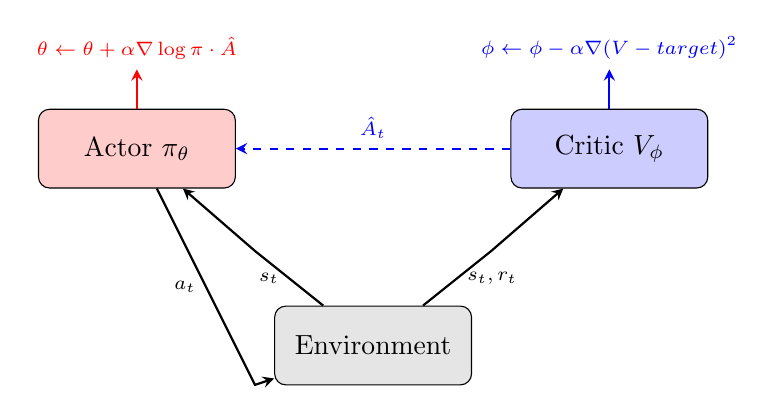
\begin{tikzpicture}[>=stealth, box/.style={rectangle, draw, rounded corners, minimum width=2.5cm, minimum height=1cm}]
        % Environment
        \node[box, fill=gray!20] (env) at (0,0) {Environment};

        % Actor
        \node[box, fill=red!20] (actor) at (-3, 2.5) {Actor $\pi_\theta$};

        % Critic
        \node[box, fill=blue!20] (critic) at (3, 2.5) {Critic $V_\phi$};

        % Arrows
        \draw[->, thick] (env) -- node[left, font=\scriptsize] {$s_t$} (-1.5, 1.2) -- (actor);
        \draw[->, thick] (env) -- node[right, font=\scriptsize] {$s_t, r_t$} (1.5, 1.2) -- (critic);
        \draw[->, thick] (actor) -- node[left, font=\scriptsize] {$a_t$} (-1.5, -0.5) -- (env);

        % Critic to Actor
        \draw[->, thick, dashed, blue] (critic) -- node[above, font=\scriptsize] {$\hat{A}_t$} (actor);

        % Update arrows
        \draw[->, thick, red] (actor.north) -- ++(0, 0.5) node[above, font=\scriptsize] {$\theta \leftarrow \theta + \alpha \nabla \log \pi \cdot \hat{A}$};
        \draw[->, thick, blue] (critic.north) -- ++(0, 0.5) node[above, font=\scriptsize] {$\phi \leftarrow \phi - \alpha \nabla (V - \text{target})^2$};
    \end{tikzpicture}
\end{center}

\begin{remark}[Why Actor-Critic?]
    \begin{center}
        \begin{tabular}{l|ccc}
                               & \textbf{REINFORCE} & \textbf{Actor-Critic} & \textbf{Pure Critic (DQN)} \\
            \hline
            Variance           & High               & Low                   & N/A                        \\
            Bias               & None               & Some (from $V$)       & None                       \\
            Continuous actions & Yes                & Yes                   & No                         \\
            Sample efficiency  & Low                & Medium                & High                       \\
        \end{tabular}
    \end{center}
\end{remark}

\subsection{Generalized Advantage Estimation (GAE)}

GAE provides a practical way to estimate advantages with controllable bias-variance tradeoff.

\begin{definition}[Generalized Advantage Estimation]
    Given TD errors $\delta_t = r_t + \gamma V(s_{t+1}) - V(s_t)$, the GAE estimator is:
    \[
        \hat{A}_t^{\text{GAE}(\gamma, \lambda)} = \sum_{l=0}^{\infty} (\gamma \lambda)^l \delta_{t+l} = \delta_t + \gamma \lambda \delta_{t+1} + (\gamma \lambda)^2 \delta_{t+2} + \cdots
    \]
    where $\lambda \in [0,1]$ controls bias-variance tradeoff.
\end{definition}

\begin{remark}[GAE Special Cases]
    \begin{itemize}
        \item $\lambda = 0$: $\hat{A}_t = \delta_t = r_t + \gamma V(s_{t+1}) - V(s_t)$ (1-step TD, high bias, low variance)
        \item $\lambda = 1$: $\hat{A}_t = \sum_{l=0}^{\infty} \gamma^l \delta_{t+l} = G_t - V(s_t)$ (Monte Carlo, no bias, high variance)
    \end{itemize}
    In practice, $\lambda \approx 0.95$ works well---enough bootstrapping to reduce variance, but not so much that bias dominates.
\end{remark}

\begin{center}
    \begin{tikzpicture}[>=stealth]
        % Timeline
        \draw[thick] (0,0) -- (12,0);

        % States and deltas
        \foreach \i in {0,1,2,3,4} {
                \node[circle, draw, fill=blue!20, minimum size=6mm, font=\scriptsize] (s\i) at (2.4*\i, 0) {$s_{t+\i}$};
            }

        % Delta labels
        \foreach \i/\next in {0/1, 1/2, 2/3, 3/4} {
                \draw[->, thick] (s\i) -- node[above, font=\scriptsize] {$\delta_{t+\i}$} (s\next);
            }

        % GAE sum visualization
        \node[below=1.5cm of s0, font=\small] {$\hat{A}_t^{\text{GAE}} = \delta_t$};
        \node[below=1.5cm of s1, font=\small] {$+ \gamma\lambda \delta_{t+1}$};
        \node[below=1.5cm of s2, font=\small] {$+ (\gamma\lambda)^2 \delta_{t+2}$};
        \node[below=1.5cm of s3, font=\small] {$+ \cdots$};

        % Weights visualization
        \draw[thick, red, opacity=0.6] (0, -0.5) rectangle (0.8, -0.3);
        \draw[thick, red, opacity=0.4] (2.4, -0.5) rectangle (2.9, -0.3);
        \draw[thick, red, opacity=0.25] (4.8, -0.5) rectangle (5.15, -0.3);
        \draw[thick, red, opacity=0.15] (7.2, -0.5) rectangle (7.4, -0.3);

        \node[right, font=\scriptsize, red] at (8, -0.4) {weights decay as $(\gamma\lambda)^l$};
    \end{tikzpicture}
\end{center}

\begin{proposition}[GAE as Exponentially-Weighted Average]
    GAE can be written as:
    \[
        \hat{A}_t^{\text{GAE}} = (1-\lambda) \sum_{n=1}^{\infty} \lambda^{n-1} \hat{A}_t^{(n)}
    \]
    where $\hat{A}_t^{(n)} = \sum_{l=0}^{n-1} \gamma^l r_{t+l} + \gamma^n V(s_{t+n}) - V(s_t)$ is the $n$-step advantage estimate. This shows GAE averages over all $n$-step estimates, with exponentially decaying weights.
\end{proposition}

\section{Proximal Policy Optimization (PPO)}

\begin{definition}[Proximal Policy Optimization]
    Proximal Policy Optimization (PPO) is a first-order policy gradient algorithm that still aims to maximize the true return $J(\theta)$ but \emph{actually} optimizes a clipped surrogate objective $\mathcal{L}^{\text{PPO}}(\theta)$ (defined below) using samples from $\pi_{\theta_{\text{old}}}$.
    It constrains the change between the new policy $\pi_\theta$ and the data-collecting policy $\pi_{\theta_{\text{old}}}$ (via probability-ratio clipping or an explicit KL penalty), allowing relatively large learning rates while keeping updates stable.
    In practice, PPO alternates between (i) collecting trajectories with $\pi_{\theta_{\text{old}}}$ and (ii) several epochs of gradient ascent on $\mathcal{L}^{\text{PPO}}$ using minibatches.
\end{definition}

\subsection{The Problem with Vanilla Policy Gradient}

Recall the policy gradient objective $J(\theta) = \mathbb{E}_{\tau \sim \pi_\theta}[R(\tau)]$. The gradient tells us how to improve:
\[
    \nabla_\theta J(\theta) = \mathbb{E}_t \left[ \nabla_\theta \log \pi_\theta(a_t|s_t) \cdot A_t \right]
\]
where $A_t$ is the advantage (how much better action $a_t$ was than average).

\textbf{Problem}: Gradient descent takes a step $\theta \to \theta + \alpha \nabla_\theta J$. But how big should $\alpha$ be? Too small = slow. Too large = policy changes drastically, samples become invalid, training collapses.

\textbf{Answer}: control the \emph{size of the policy change}, not just the learning rate. Trust-region style methods bound the KL divergence between $\pi_\theta$ and $\pi_{\theta_{\text{old}}}$ so that updates stay within a region where old samples are still informative. PPO implements this idea with a clipped surrogate (and optionally a KL penalty), which effectively caps the probability ratio $r_t(\theta)$ so a large $\alpha$ cannot cause destructive jumps. In practice one still uses an optimizer like Adam, but clipping/penalty provides the main safeguard.

\subsection{The Importance Sampling Trick}

We want to reuse data collected under an old policy $\pi_{\theta_{\text{old}}}$ to improve a new policy $\pi_\theta$. Using importance sampling:
\[
    \mathbb{E}_{a \sim \pi_\theta}\bigl[f(a)\bigr] = \mathbb{E}_{a \sim \pi_{\theta_{\text{old}}}}\left[ \frac{\pi_\theta(a|s)}{\pi_{\theta_{\text{old}}}(a|s)} f(a) \right].
\]

\begin{definition}[Probability Ratio]
    The probability ratio measures how much more (or less) likely action $a_t$ is under the new policy compared to the old:
    \[
        r_t(\theta) = \frac{\pi_\theta(a_t|s_t)}{\pi_{\theta_{\text{old}}}(a_t|s_t)}.
    \]
    \begin{itemize}
        \item $r_t = 1$: new and old policies agree on this action
        \item $r_t > 1$: new policy makes this action \emph{more} likely
        \item $r_t < 1$: new policy makes this action \emph{less} likely
    \end{itemize}
\end{definition}

Using this ratio, we can write a \emph{policy-gradient surrogate} that we optimize using data from $\pi_{\theta_{\text{old}}}$:
\[
    \mathcal{L}^{\text{PG}}(\theta) = \mathbb{E}_t \left[ r_t(\theta) \cdot A_t \right].
\]
This equals $J(\theta)$ to first order around $\theta_{\text{old}}$, but can be computed using old samples.

\subsection{Why We Need Clipping}

The problem: if $r_t(\theta)$ becomes very large, the surrogate $\mathcal{L}^{\text{PG}}(\theta) = \mathbb{E}[r_t A_t]$ gives huge gradients, causing destructive updates. We want to constrain how far the new policy can drift from the old one.

\begin{definition}[PPO-Clip Objective]
    \[
        \mathcal{L}^{\text{PPO}}(\theta) = \mathbb{E}_t \left[ \min\left( r_t(\theta) \cdot A_t, \; \text{clip}(r_t(\theta), 1-\epsilon, 1+\epsilon) \cdot A_t \right) \right]
    \]
    where $\epsilon \approx 0.2$ and $\text{clip}(r, 1-\epsilon, 1+\epsilon)$ clamps $r$ to $[1-\epsilon, 1+\epsilon]$.
\end{definition}

\begin{remark}[How Clipping Works]
    The clipping behaves differently depending on whether the action was good ($A_t > 0$) or bad ($A_t < 0$):

    \textbf{Case 1: Good action ($A_t > 0$)}
    \begin{itemize}
        \item If $r_t < 1 - \epsilon$: action became less likely. Gradient pushes to increase $r_t$.
        \item If $r_t \in [1-\epsilon, 1+\epsilon]$: normal gradient, objective is $r_t \cdot A_t$.
        \item If $r_t > 1 + \epsilon$: action became much more likely. The $\min$ kicks in, objective becomes $(1+\epsilon) A_t$---flat, no gradient to increase $r_t$ further.
    \end{itemize}

    \textbf{Case 2: Bad action ($A_t < 0$)}
    \begin{itemize}
        \item If $r_t > 1 + \epsilon$: action became more likely (bad!). Gradient pushes to decrease $r_t$.
        \item If $r_t \in [1-\epsilon, 1+\epsilon]$: normal gradient, objective is $r_t \cdot A_t$ (negative).
        \item If $r_t < 1 - \epsilon$: action became much less likely. The $\min$ kicks in (clipped value is less negative), objective becomes $(1-\epsilon) A_t$---flat, no further decrease.
    \end{itemize}
\end{remark}

\begin{center}
    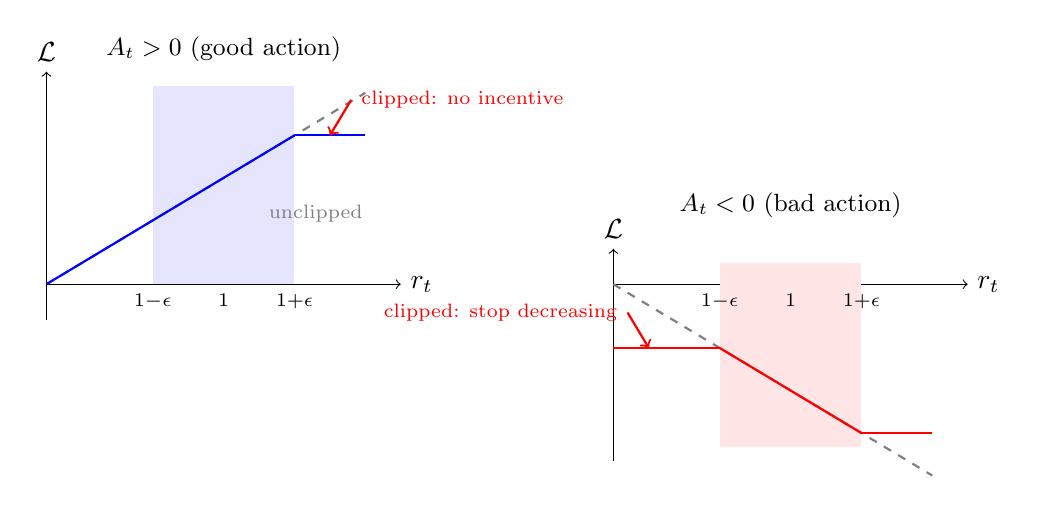
\begin{tikzpicture}[scale=0.9]
        % Left plot: A > 0
        \begin{scope}[shift={(-5,0)}]
            \draw[->] (0,0) -- (5,0) node[right] {$r_t$};
            \draw[->] (0,-0.5) -- (0,3) node[above] {$\mathcal{L}$};

            % Clip region
            \fill[blue!10] (1.5,0) rectangle (3.5,2.8);

            % Unclipped line
            \draw[thick, gray, dashed] (0,0) -- (4.5, 2.7);

            % Clipped objective
            \draw[thick, blue] (0,0) -- (1.5, 0.9);
            \draw[thick, blue] (1.5, 0.9) -- (3.5, 2.1);
            \draw[thick, blue] (3.5, 2.1) -- (4.5, 2.1);

            % Labels
            \node[below] at (1.5,0) {\scriptsize $1{-}\epsilon$};
            \node[below] at (3.5,0) {\scriptsize $1{+}\epsilon$};
            \node[below] at (2.5,0) {\scriptsize $1$};

            \node[above, font=\small] at (2.5, 3) {$A_t > 0$ (good action)};

            % Annotations
            \draw[<-, thick, red] (4, 2.1) -- (4.3, 2.6) node[right, font=\scriptsize] {clipped: no incentive};
            \node[font=\scriptsize, gray] at (3.8, 1) {unclipped};
        \end{scope}

        % Right plot: A < 0
        \begin{scope}[shift={(3,0)}]
            \draw[->] (0,0) -- (5,0) node[right] {$r_t$};
            \draw[->] (0,-2.5) -- (0,0.5) node[above] {$\mathcal{L}$};

            % Clip region
            \fill[red!10] (1.5,-2.3) rectangle (3.5,0.3);

            % Unclipped line
            \draw[thick, gray, dashed] (0,0) -- (4.5, -2.7);

            % Clipped objective
            \draw[thick, red] (0,-0.9) -- (1.5, -0.9);
            \draw[thick, red] (1.5, -0.9) -- (3.5, -2.1);
            \draw[thick, red] (3.5, -2.1) -- (4.5, -2.1);

            % Labels
            \node[below] at (1.5,0) {\scriptsize $1{-}\epsilon$};
            \node[below] at (3.5,0) {\scriptsize $1{+}\epsilon$};
            \node[below] at (2.5,0) {\scriptsize $1$};

            \node[above, font=\small] at (2.5, 0.8) {$A_t < 0$ (bad action)};

            % Annotations
            \draw[<-, thick, red] (0.5, -0.9) -- (0.2, -0.4) node[left, font=\scriptsize] {clipped: stop decreasing};
        \end{scope}
    \end{tikzpicture}
\end{center}

\begin{remark}[The Pessimistic Bound]
    The $\min$ in PPO is \emph{pessimistic}---it takes the lower of the clipped and unclipped objectives. This ensures:
    \begin{itemize}
        \item We never get ``credit'' for making a good action too likely ($r_t > 1+\epsilon$).
        \item We never get ``credit'' for making a bad action too unlikely ($r_t < 1-\epsilon$).
    \end{itemize}
    The effect: the policy can improve within the trust region, but cannot exploit the surrogate objective by moving too far.
\end{remark}

\begin{remark}[Notation: $J$ vs $\mathcal{L}$]
    $J(\theta)$ is the true objective we want to maximize. $\mathcal{L}^{\text{PG}}(\theta)$ and $\mathcal{L}^{\text{PPO}}(\theta)$ are \emph{surrogate} objectives that:
    \begin{enumerate}
        \item Can be computed from samples collected under $\pi_{\theta_{\text{old}}}$
        \item Approximates $J(\theta)$ near $\theta_{\text{old}}$
        \item Has safety mechanisms (clipping) to prevent bad updates
    \end{enumerate}
    Workflow: collect samples with current policy, optimize $\mathcal{L}^{\text{PPO}}$ (the clipped surrogate), update policy, repeat. Keep $J$ for the true return, and use $\mathcal{L}$ symbols only for surrogate training objectives to avoid notational whiplash.
\end{remark}

\begin{remark}[PPO in RLHF]
    PPO is the algorithm typically used for the ``RL Fine-Tuning'' stage of RLHF (\cref{ch:rl-for-llms}). The connection:
    \begin{itemize}
        \item \textbf{Policy}: $\pi_\theta$ is the language model being fine-tuned.
        \item \textbf{Reward}: $r_\phi(x,y)$ is the learned reward model (plus KL penalty).
        \item \textbf{Advantage}: Estimated from generated responses using GAE or simpler baselines.
        \item \textbf{Clipping}: Prevents the LLM from changing too drastically in one update.
    \end{itemize}
    The PPO objective becomes:
    \[
        \mathcal{L}(\theta) = \mathbb{E}_{x, y \sim \pi_{\theta_{\text{old}}}} \left[ \min\left( \frac{\pi_\theta(y|x)}{\pi_{\theta_{\text{old}}}(y|x)} \hat{A}, \; \text{clip}(\cdot) \cdot \hat{A} \right) \right]
    \]
    where $\hat{A}$ incorporates the reward $r_\phi(x,y)$ and KL penalty $-\beta \log \frac{\pi_\theta(y|x)}{\pi_{\text{ref}}(y|x)}$.

    \textbf{Note}: PPO's clipping and RLHF's KL penalty both serve to keep the policy from drifting too far---they're complementary regularization mechanisms.
\end{remark}

% ============================================================
\chapter{Reinforcement Learning for Language Models}
\label{ch:rl-for-llms}

This chapter applies RL to language models, where the goal is to align model outputs with human preferences. The MDP structure from \cref{ch:classical-rl} still applies, but with important differences:

\begin{remark}[LLMs as MDPs]
    For a language model generating response $y = (y_1, y_2, \ldots, y_T)$ to prompt $x$:
    \begin{itemize}
        \item \textbf{State}: $s_t = (x, y_1, \ldots, y_{t-1})$ --- the prompt plus tokens generated so far.
        \item \textbf{Action}: $a_t = y_t$ --- the next token to generate.
        \item \textbf{Policy}: $\pi_\theta(a_t | s_t) = \pi_\theta(y_t | x, y_{<t})$ --- the LLM's next-token distribution.
        \item \textbf{Transition}: $P(s_{t+1}|s_t, a_t) = 1$ --- \emph{deterministic}! The next state is just $(x, y_1, \ldots, y_t)$.
        \item \textbf{Reward}: Often given only at the end: $R(s_T, a_T) = r_\phi(x, y)$, with $R(s_t, a_t) = 0$ for $t < T$.
    \end{itemize}
\end{remark}

\begin{remark}[Key Differences from Classical RL]
    \textbf{1. Deterministic environment.} In robotics, the same action leads to different outcomes due to physics. In LLMs, appending token $y_t$ to state $s_t$ always gives the same next state. All randomness comes from the policy.

    \textbf{2. Sparse, delayed reward.} Classical RL often has dense rewards (e.g., distance to goal at each step). LLM rewards are typically given only after the full response---the reward model $r_\phi(x,y)$ evaluates complete outputs.

    \textbf{3. No simulator.} We cannot reset to arbitrary states or query the reward function cheaply. Each sample requires a forward pass through the LLM.

    \textbf{4. The reference policy matters.} Unlike classical RL where we start from random initialization, LLMs begin with a pre-trained model that already has useful behavior. We want to \emph{improve} upon it, not destroy it. This motivates the KL constraint in RLHF.

    \textbf{5. Preference data, not reward labels.} Humans find it easier to compare ``Is response A better than B?'' than to assign absolute scores. This leads to preference-based methods (Bradley-Terry, DPO).
\end{remark}

\section{RLHF: Reinforcement Learning from Human Feedback}

Fine-tuning language models with RL proceeds in three stages:
\begin{enumerate}
    \item \textbf{Supervised Fine-Tuning (SFT)}: Train on high-quality demonstrations.
    \item \textbf{Reward Modeling}: Train a reward model $r_\phi(x, y)$ on human preference data.
    \item \textbf{RL Fine-Tuning}: Optimize the policy against the reward model.
\end{enumerate}

\begin{center}
    \begin{tikzpicture}[
            >=stealth,
            stage/.style={rectangle, draw, rounded corners, minimum width=3cm, minimum height=1.2cm, align=center},
            data/.style={rectangle, draw, dashed, minimum width=2.5cm, minimum height=0.8cm, align=center, font=\scriptsize},
            arrow/.style={->, thick}
        ]
        % Stage 1: SFT
        \node[stage, fill=green!20] (sft) at (0, 0) {Stage 1:\\SFT};
        \node[data, above=0.5cm of sft] (sft_data) {Demonstrations\\$(x, y^*)$};
        \node[below=0.3cm of sft, font=\scriptsize] {$\pi_{\text{ref}} = \pi_{\text{SFT}}$};

        % Stage 2: Reward Model
        \node[stage, fill=blue!20] (rm) at (5, 0) {Stage 2:\\Reward Model};
        \node[data, above=0.5cm of rm] (rm_data) {Preferences\\$(x, y_w \succ y_l)$};
        \node[below=0.3cm of rm, font=\scriptsize] {$r_\phi(x, y)$};

        % Stage 3: RL
        \node[stage, fill=red!20] (rl) at (10, 0) {Stage 3:\\RL Fine-Tuning};
        \node[data, above=0.5cm of rl] (rl_data) {Prompts\\$x \sim \mathcal{D}$};
        \node[below=0.3cm of rl, font=\scriptsize] {$\pi_\theta$};

        % Arrows between stages
        \draw[arrow] (sft) -- node[above, font=\scriptsize] {init} (rm);
        \draw[arrow] (rm) -- node[above, font=\scriptsize] {reward} (rl);

        % Feedback loop in RL
        \draw[arrow, red] (rl.south) -- ++(0, -0.8) -| node[below, pos=0.25, font=\scriptsize] {sample $y \sim \pi_\theta$, score with $r_\phi$} (rl.south west);

        % Data arrows
        \draw[arrow, dashed] (sft_data) -- (sft);
        \draw[arrow, dashed] (rm_data) -- (rm);
        \draw[arrow, dashed] (rl_data) -- (rl);

        % Human label for preferences
        \node[above=0.3cm of rm_data, font=\scriptsize] {Human labelers};
    \end{tikzpicture}
\end{center}

\begin{remark}[Data Requirements]
    Each stage requires different data:
    \begin{center}
        \begin{tabular}{l|l|l}
            \textbf{Stage} & \textbf{Data Type}                       & \textbf{Typical Size} \\
            \hline
            SFT            & High-quality $(x, y)$ pairs              & 10K--100K             \\
            Reward Model   & Preference comparisons $(y_w \succ y_l)$ & 10K--500K             \\
            RL             & Prompts only (responses sampled)         & 10K--100K             \\
        \end{tabular}
    \end{center}
\end{remark}

\subsection{The RLHF Objective}

\begin{definition}[RLHF Objective]
    Given a prompt $x$, the objective is to maximize reward while staying close to the reference policy $\pi_{\text{ref}}$ (typically the SFT model):
    \[
        \max_{\pi_\theta} \; \mathbb{E}_{x \sim \mathcal{D}, \, y \sim \pi_\theta(\cdot|x)} \left[ r_\phi(x, y) - \beta \, D_{\mathrm{KL}}\bigl(\pi_\theta(\cdot|x) \,\|\, \pi_{\text{ref}}(\cdot|x)\bigr) \right].
    \]
\end{definition}

\begin{example}[RLHF in Action]
    Prompt: $x$ = ``Explain why the sky is blue.''

    The policy $\pi_\theta(\cdot|x)$ is a distribution over all possible responses. For illustration, suppose there are only 3 possible outputs:
    \begin{center}
        \begin{tabular}{l|cc|c}
            Response $y$                       & $\pi_\theta(y|x)$ & $\pi_{\text{ref}}(y|x)$ & $r_\phi(x,y)$ \\
            \hline
            $y_1$: ``Rayleigh scattering...''  & 0.50              & 0.40                    & 0.9           \\
            $y_2$: ``The sky appears blue...'' & 0.45              & 0.35                    & 0.85          \\
            $y_3$: ``Blue blue blue...''       & 0.05              & 0.25                    & 0.1           \\
        \end{tabular}
    \end{center}

    \textbf{Notation}: $\pi_\theta(y_1|x) = 0.50$ is a number. $\pi_\theta(\cdot|x) = (0.50, 0.45, 0.05)$ is the entire distribution.

    \textbf{Computing the KL divergence}:
    \[
        D_{\mathrm{KL}}\bigl(\pi_\theta(\cdot|x) \,\|\, \pi_{\text{ref}}(\cdot|x)\bigr) = \sum_{y} \pi_\theta(y|x) \log \frac{\pi_\theta(y|x)}{\pi_{\text{ref}}(y|x)}.
    \]
    With our numbers:
    \begin{align*}
        D_{\mathrm{KL}} & = 0.50 \log\frac{0.50}{0.40} + 0.45 \log\frac{0.45}{0.35} + 0.05 \log\frac{0.05}{0.25} \\
                        & = 0.50 \cdot 0.223 + 0.45 \cdot 0.251 + 0.05 \cdot (-1.609)                            \\
                        & = 0.112 + 0.113 - 0.080 = 0.145.
    \end{align*}
    The KL is positive because $\pi_\theta$ shifted probability \emph{toward} good responses ($y_1, y_2$) and \emph{away from} the bad one ($y_3$).

    \textbf{The full objective} for this prompt:
    \[
        \underbrace{0.50 \cdot 0.9 + 0.45 \cdot 0.85 + 0.05 \cdot 0.1}_{\mathbb{E}_{y \sim \pi_\theta}[r_\phi(x,y)] = 0.838} - \beta \cdot \underbrace{0.145}_{D_{\mathrm{KL}}}.
    \]
    If $\beta = 0.1$, the objective is $0.838 - 0.0145 = 0.824$. The reward term wants to push even more probability to $y_1$, but the KL term resists moving too far from $\pi_{\text{ref}}$.
\end{example}

\begin{remark}[How RLHF Works in Practice]
    The example above is a simplification. In reality:

    \textbf{1. Where do responses come from?}
    We \emph{sample} from the policy: $y \sim \pi_\theta(\cdot|x)$. This means running the LLM autoregressively, sampling one token at a time. We do \emph{not} use beam search---we need stochastic samples because RL requires exploring different outputs. Typically we sample $k$ responses per prompt (e.g., $k=4$).

    \textbf{2. Who assigns the rewards?}
    The reward model $r_\phi(x, y)$---a neural network trained on human preference data. During reward model training, humans compared pairs of responses and labeled which was better. The reward model learned to predict these preferences.

    \textbf{3. How do we compute $D_{\mathrm{KL}}$ without enumerating all responses?}
    We cannot sum over all possible $y$---the space is astronomically large. Instead, rewrite the KL as an expectation:
    \[
        D_{\mathrm{KL}}\bigl(\pi_\theta \| \pi_{\text{ref}}\bigr) = \mathbb{E}_{y \sim \pi_\theta(\cdot|x)} \left[ \log \frac{\pi_\theta(y|x)}{\pi_{\text{ref}}(y|x)} \right] = \mathbb{E}_{y \sim \pi_\theta} \left[ \log \pi_\theta(y|x) - \log \pi_{\text{ref}}(y|x) \right].
    \]
    For a \emph{single sample} $y \sim \pi_\theta(\cdot|x)$, the quantity $\log \pi_\theta(y|x) - \log \pi_{\text{ref}}(y|x)$ is an unbiased estimate of the KL.

    \textbf{Computing $\log \pi_\theta(y|x)$}: For an LLM, this is just the sum of log-probabilities of each token:
    \[
        \log \pi_\theta(y|x) = \sum_{t=1}^{T} \log \pi_\theta(y_t | x, y_{<t}).
    \]
    Run the LLM on the response, read off the probability it assigns to each token, sum the logs. Do this for both $\pi_\theta$ and $\pi_{\text{ref}}$, subtract.
\end{remark}

\begin{remark}[Why the KL Penalty?]
    Without the KL term, we would simply maximize $\mathbb{E}[r_\phi(x,y)]$. This fails for several reasons:
    \begin{enumerate}
        \item \textbf{Reward hacking}: The reward model $r_\phi$ is imperfect---trained on limited data. The policy will find adversarial outputs that score high on $r_\phi$ but are actually garbage. Example: repetitive text, nonsense that exploits quirks in the reward model.

        \item \textbf{Distribution shift}: The reward model was trained on outputs from $\pi_{\text{ref}}$. As $\pi_\theta$ drifts away, $r_\phi$'s predictions become unreliable (it's being evaluated out-of-distribution).

        \item \textbf{Mode collapse}: Without regularization, the policy might converge to always outputting the same high-reward response, losing diversity.

        \item \textbf{Preserve capabilities}: $\pi_{\text{ref}}$ (the SFT model) already produces coherent, grammatical text. We want to improve \emph{alignment}, not destroy language ability.
    \end{enumerate}
    The KL term acts as a ``leash''---the policy can improve, but not wander too far from known-good behavior.
\end{remark}

\begin{remark}[KL Divergence Direction: Why $D_{\mathrm{KL}}(\pi_\theta \| \pi_{\text{ref}})$?]
    The KL divergence is \emph{asymmetric}: $D_{\mathrm{KL}}(P \| Q) \neq D_{\mathrm{KL}}(Q \| P)$. The two directions have different names and behaviors:

    \begin{definition}[KL Divergence Directions]
        For distributions $P$ and $Q$:
        \begin{align*}
            \textbf{Forward KL:} \quad D_{\mathrm{KL}}(P \| Q) & = \mathbb{E}_{x \sim P}\left[\log \frac{P(x)}{Q(x)}\right] \quad \text{(expectation under $P$)} \\[6pt]
            \textbf{Reverse KL:} \quad D_{\mathrm{KL}}(Q \| P) & = \mathbb{E}_{x \sim Q}\left[\log \frac{Q(x)}{P(x)}\right] \quad \text{(expectation under $Q$)}
        \end{align*}
        The naming convention: $P$ is the ``target'' or ``true'' distribution, $Q$ is the ``approximation.''
    \end{definition}

    In RLHF, $\pi_{\text{ref}}$ is the reference (playing the role of $P$) and $\pi_\theta$ is what we're learning (playing the role of $Q$). We use:
    \[
        D_{\mathrm{KL}}(\underbrace{\pi_\theta}_{Q} \| \underbrace{\pi_{\text{ref}}}_{P}) = \mathbb{E}_{y \sim \pi_\theta}\left[\log \frac{\pi_\theta(y|x)}{\pi_{\text{ref}}(y|x)}\right] \quad \textbf{(Reverse KL: $D_{\mathrm{KL}}(Q \| P)$)}
    \]
    This is reverse KL because the \textbf{expectation is taken under $\pi_\theta$} (the distribution we're learning), not under $\pi_{\text{ref}}$ (the reference).

    \textbf{Why does RLHF use reverse KL?} The two directions have very different behaviors:

    \begin{center}
        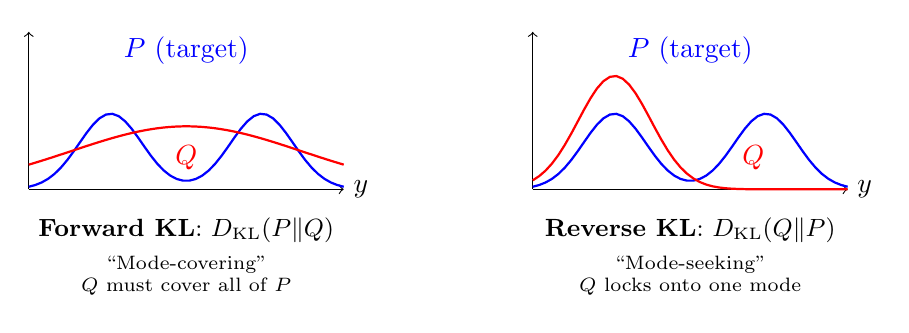
\begin{tikzpicture}[scale=0.8]
            % Forward KL
            \begin{scope}[shift={(-4,0)}]
                \draw[->] (0,0) -- (5,0) node[right] {$y$};
                \draw[->] (0,0) -- (0,2.5);

                % Target P (bimodal)
                \draw[thick, blue, domain=0:5, samples=50] plot (\x, {1.2*exp(-2*(\x-1.3)^2) + 1.2*exp(-2*(\x-3.7)^2)});
                \node[blue] at (2.5, 2.2) {$P$ (target)};

                % Approximation Q (wide, covers both)
                \draw[thick, red, domain=0:5, samples=50] plot (\x, {1.0*exp(-0.15*(\x-2.5)^2)});
                \node[red] at (2.5, 0.5) {$Q$};

                \node[below, font=\small, align=center] at (2.5, -0.3) {\textbf{Forward KL}: $D_{\mathrm{KL}}(P \| Q)$};
                \node[below, font=\scriptsize, align=center] at (2.5, -0.9) {``Mode-covering''\\$Q$ must cover all of $P$};
            \end{scope}

            % Reverse KL
            \begin{scope}[shift={(4,0)}]
                \draw[->] (0,0) -- (5,0) node[right] {$y$};
                \draw[->] (0,0) -- (0,2.5);

                % Target P (bimodal)
                \draw[thick, blue, domain=0:5, samples=50] plot (\x, {1.2*exp(-2*(\x-1.3)^2) + 1.2*exp(-2*(\x-3.7)^2)});
                \node[blue] at (2.5, 2.2) {$P$ (target)};

                % Approximation Q (narrow, picks one mode)
                \draw[thick, red, domain=0:5, samples=50] plot (\x, {1.8*exp(-1.5*(\x-1.3)^2)});
                \node[red] at (3.5, 0.5) {$Q$};

                \node[below, font=\small, align=center] at (2.5, -0.3) {\textbf{Reverse KL}: $D_{\mathrm{KL}}(Q \| P)$};
                \node[below, font=\scriptsize, align=center] at (2.5, -0.9) {``Mode-seeking''\\$Q$ locks onto one mode};
            \end{scope}
        \end{tikzpicture}
    \end{center}

    \begin{itemize}
        \item \textbf{Forward KL} $D_{\mathrm{KL}}(P \| Q)$: Expectation under $P$. Penalizes $Q$ whenever $P(x) > 0$ but $Q(x) \approx 0$. Effect: $Q$ must \emph{cover} all modes of $P$, even if it means spreading mass where $P$ is low. This is \textbf{mode-covering} (also called ``mean-seeking'' or ``inclusive'').

        \item \textbf{Reverse KL} $D_{\mathrm{KL}}(Q \| P)$: Expectation under $Q$. Penalizes $Q$ whenever $Q(x) > 0$ but $P(x) \approx 0$. Effect: $Q$ avoids placing mass where $P$ is low, typically \emph{locking onto} a single mode of $P$. This is \textbf{mode-seeking} (also called ``zero-forcing'' or ``exclusive'').
    \end{itemize}

    \textbf{In RLHF}, we use reverse KL $D_{\mathrm{KL}}(\pi_\theta \| \pi_{\text{ref}})$ because:
    \begin{enumerate}
        \item The expectation is under $\pi_\theta$, which we can sample from (we generate from the policy).
        \item Mode-seeking behavior is desirable: we want $\pi_\theta$ to concentrate on high-quality outputs rather than spreading probability to cover everything $\pi_{\text{ref}}$ might generate.
        \item If $\pi_\theta$ tries to put mass where $\pi_{\text{ref}}$ has near-zero probability, the penalty $\log(\pi_\theta / \pi_{\text{ref}}) \to +\infty$ explodes. This prevents the policy from generating outputs that the reference model would never produce.
    \end{enumerate}
\end{remark}

\begin{remark}[When to Question the KL Penalty]
    The KL penalty is not always the right choice:
    \begin{enumerate}
        \item \textbf{Over-regularization}: If $\beta$ is too large, the model barely moves from $\pi_{\text{ref}}$. You pay the cost of RL but get minimal improvement. Some tasks genuinely require the model to behave very differently from the SFT baseline.

        \item \textbf{Bad reference policy}: If $\pi_{\text{ref}}$ is itself flawed (e.g., trained on low-quality data), anchoring to it perpetuates those flaws.

        \item \textbf{Tuning $\beta$ is hard}: Too small = reward hacking. Too large = no learning. The optimal $\beta$ depends on the task, reward model quality, and is often found by expensive hyperparameter search.

        \item \textbf{Alternative regularization}: Methods like GRPO use group-based normalization instead of KL, arguing that relative ranking within a batch is more robust than absolute distance from a reference.
    \end{enumerate}
\end{remark}

\subsection{Reward Modeling}

The key insight: humans are better at \emph{comparing} options than assigning absolute scores. Instead of asking ``Rate this response 1-10,'' we ask ``Which response is better?''

\begin{remark}[Why Bradley-Terry?]
    The Bradley-Terry model (1952) was originally developed for ranking chess players. The idea: each player has an underlying ``strength'' $s_i$, and the probability that player $i$ beats player $j$ is:
    \[
        P(i \text{ beats } j) = \frac{s_i}{s_i + s_j} = \frac{1}{1 + s_j/s_i} = \sigma\left(\log \frac{s_i}{s_j}\right) = \sigma(\log s_i - \log s_j).
    \]
    If we define $r_i = \log s_i$ as the ``rating,'' we get $P(i \text{ beats } j) = \sigma(r_i - r_j)$.

    \textbf{Key properties:}
    \begin{itemize}
        \item \emph{Transitivity}: If $r_A > r_B > r_C$, then $P(A \succ B) > 0.5$ and $P(B \succ C) > 0.5$.
        \item \emph{Invariance}: Only \emph{differences} in reward matter, not absolute values. Adding a constant to all rewards doesn't change preferences.
        \item \emph{Calibration}: When $r_w - r_l = 0$, we get $P = 0.5$ (tie). As the difference grows, $P \to 1$.
    \end{itemize}

    For LLMs, we replace player strength with response quality: $r_\phi(x, y)$ is the ``reward'' or quality score for response $y$ to prompt $x$.
\end{remark}

\begin{definition}[Bradley-Terry Model]
    Given preference pairs $(y_w, y_l)$ where $y_w$ is preferred over $y_l$, the probability of the preference under the Bradley-Terry model is
    \[
        P(y_w \succ y_l | x) = \sigma\bigl(r_\phi(x, y_w) - r_\phi(x, y_l)\bigr)
    \]
    where $\sigma(z) = 1/(1 + e^{-z})$ is the sigmoid function.
\end{definition}

\begin{definition}[Reward Model Loss]
    The reward model is trained to minimize the negative log-likelihood:
    \[
        \mathcal{L}_{\text{RM}}(\phi) = -\mathbb{E}_{(x, y_w, y_l) \sim \mathcal{D}} \left[ \log \sigma\bigl(r_\phi(x, y_w) - r_\phi(x, y_l)\bigr) \right].
    \]
\end{definition}

\section{DPO: Direct Preference Optimization}

DPO eliminates the need for a separate reward model by directly optimizing the policy on preference data.

\subsection{Derivation}

\begin{proposition}[Optimal Policy under KL Constraint]
    The optimal policy for the RLHF objective has closed form:
    \[
        \pi^*(y|x) = \frac{1}{Z(x)} \pi_{\text{ref}}(y|x) \exp\left( \frac{r(x,y)}{\beta} \right)
    \]
    where $Z(x) = \sum_y \pi_{\text{ref}}(y|x) \exp(r(x,y)/\beta)$ is the partition function.
\end{proposition}

\begin{proof}
    The RLHF objective with KL constraint is:
    \[
        \max_\pi \; \mathbb{E}_{y \sim \pi}[r(x,y)] - \beta \, D_{\mathrm{KL}}(\pi \| \pi_{\text{ref}}).
    \]
    Expanding the KL divergence:
    \begin{align*}
         & = \mathbb{E}_{y \sim \pi}[r(x,y)] - \beta \mathbb{E}_{y \sim \pi}\left[ \log \frac{\pi(y|x)}{\pi_{\text{ref}}(y|x)} \right] \\
         & = \mathbb{E}_{y \sim \pi}\left[ r(x,y) - \beta \log \frac{\pi(y|x)}{\pi_{\text{ref}}(y|x)} \right].
    \end{align*}
    Taking the functional derivative with respect to $\pi(y|x)$ and setting to zero (with Lagrange multiplier for normalization) gives the Boltzmann distribution.
\end{proof}

\begin{corollary}[Implicit Reward]
    Rearranging the optimal policy, the reward can be expressed as:
    \[
        r(x, y) = \beta \log \frac{\pi^*(y|x)}{\pi_{\text{ref}}(y|x)} + \beta \log Z(x).
    \]
\end{corollary}

\begin{theorem}[DPO Loss]
    Substituting the implicit reward into the Bradley-Terry preference model, the partition functions cancel:
    \[
        \mathcal{L}_{\text{DPO}}(\theta) = -\mathbb{E}_{(x, y_w, y_l)} \left[ \log \sigma\left( \beta \log \frac{\pi_\theta(y_w|x)}{\pi_{\text{ref}}(y_w|x)} - \beta \log \frac{\pi_\theta(y_l|x)}{\pi_{\text{ref}}(y_l|x)} \right) \right].
    \]
\end{theorem}

\begin{proof}
    Under the Bradley-Terry model with the implicit reward:
    \begin{align*}
        P(y_w \succ y_l) & = \sigma(r(x, y_w) - r(x, y_l))                                                                                                                                              \\
                         & = \sigma\left( \beta \log \frac{\pi^*(y_w|x)}{\pi_{\text{ref}}(y_w|x)} + \beta \log Z(x) - \beta \log \frac{\pi^*(y_l|x)}{\pi_{\text{ref}}(y_l|x)} - \beta \log Z(x) \right) \\
                         & = \sigma\left( \beta \log \frac{\pi^*(y_w|x)}{\pi_{\text{ref}}(y_w|x)} - \beta \log \frac{\pi^*(y_l|x)}{\pi_{\text{ref}}(y_l|x)} \right).
    \end{align*}
    Replacing $\pi^*$ with the learned policy $\pi_\theta$ and taking negative log-likelihood gives the DPO loss.
\end{proof}

\begin{remark}
    The key insight is that the partition function $Z(x)$ cancels in the preference comparison, making the loss tractable without needing to compute the intractable normalization constant.
\end{remark}

\subsection{Gradient Analysis}

\begin{proposition}[DPO Gradient]
    The gradient of the DPO loss is:
    \[
        \nabla_\theta \mathcal{L}_{\text{DPO}} = -\beta \, \mathbb{E} \left[ \sigma(\hat{r}_l - \hat{r}_w) \left( \nabla_\theta \log \pi_\theta(y_w|x) - \nabla_\theta \log \pi_\theta(y_l|x) \right) \right]
    \]
    where $\hat{r}_y = \beta \log \frac{\pi_\theta(y|x)}{\pi_{\text{ref}}(y|x)}$ is the implicit reward.
\end{proposition}

\begin{remark}
    The weighting $\sigma(\hat{r}_l - \hat{r}_w)$ is high when the model incorrectly ranks the pair (assigns higher implicit reward to the losing response). This focuses learning on mistakes.
\end{remark}

\section{IPO: Identity Preference Optimization}

IPO addresses potential overfitting in DPO by using a different loss formulation.

\begin{definition}[IPO Loss]
    \[
        \mathcal{L}_{\text{IPO}}(\theta) = \mathbb{E}_{(x, y_w, y_l)} \left[ \left( \log \frac{\pi_\theta(y_w|x)}{\pi_{\text{ref}}(y_w|x)} - \log \frac{\pi_\theta(y_l|x)}{\pi_{\text{ref}}(y_l|x)} - \frac{1}{2\beta} \right)^2 \right].
    \]
\end{definition}

\begin{remark}
    IPO uses a squared loss that targets a fixed margin $1/(2\beta)$ between log-ratios, rather than pushing them apart indefinitely as in DPO.
\end{remark}

\subsection{Visualizing DPO vs IPO vs SLiC-HF}

The key difference between these methods is how their loss behaves as the margin $m = \hat{r}_w - \hat{r}_l$ (implicit reward difference) changes:

\begin{center}
    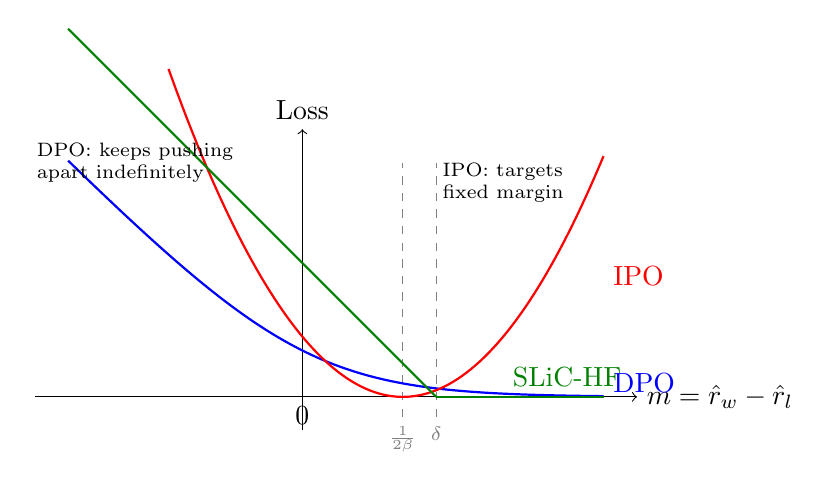
\begin{tikzpicture}[scale=0.85]
        \draw[->] (-4,0) -- (5,0) node[right] {$m = \hat{r}_w - \hat{r}_l$};
        \draw[->] (0,-0.5) -- (0,4) node[above] {Loss};

        % Target margin for IPO
        \draw[dashed, gray] (1.5, -0.3) -- (1.5, 3.5);
        \node[below, gray, font=\scriptsize] at (1.5, -0.3) {$\frac{1}{2\beta}$};

        % SLiC-HF margin
        \draw[dashed, gray] (2, -0.3) -- (2, 3.5);
        \node[below, gray, font=\scriptsize] at (2, -0.3) {$\delta$};

        % DPO: -log(sigmoid(m)) = log(1 + exp(-m))
        \draw[thick, blue, domain=-3.5:4.5, samples=100] plot (\x, {ln(1 + exp(-\x))});
        \node[blue, right] at (4.5, 0.2) {DPO};

        % IPO: (m - target)^2
        \draw[thick, red, domain=-2:4.5, samples=100] plot (\x, {0.4*(\x - 1.5)^2});
        \node[red, right] at (4.5, 1.8) {IPO};

        % SLiC-HF: max(0, delta - m)
        \draw[thick, green!50!black, domain=-3.5:2] plot (\x, {2 - \x});
        \draw[thick, green!50!black] (2,0) -- (4.5,0);
        \node[green!50!black, right] at (3, 0.3) {SLiC-HF};

        % Key points
        \node[below] at (0,0) {$0$};

        % Legend annotations
        \node[font=\scriptsize, align=left] at (-2.5, 3.5) {DPO: keeps pushing\\apart indefinitely};
        \node[font=\scriptsize, align=left] at (3, 3.2) {IPO: targets\\fixed margin};
    \end{tikzpicture}
\end{center}

\begin{remark}[Comparing Loss Behaviors]
    \begin{itemize}
        \item \textbf{DPO} ($-\log \sigma(m)$): Loss $\to 0$ as $m \to \infty$. The model is always incentivized to increase the margin further. This can lead to \emph{over-optimization}---the model keeps pushing probabilities to extremes even after the preference is satisfied.

        \item \textbf{IPO} ($(m - \frac{1}{2\beta})^2$): Loss is minimized at $m = \frac{1}{2\beta}$. Once the target margin is achieved, pushing further \emph{increases} the loss. This prevents over-optimization.

        \item \textbf{SLiC-HF} ($\max(0, \delta - m)$): Loss is exactly zero once $m \geq \delta$. No gradient once the margin is satisfied---the model stops optimizing this pair entirely.
    \end{itemize}
\end{remark}

\begin{remark}[Gradient Magnitude Comparison]
    The gradient magnitude reveals how aggressively each method learns:

    \begin{center}
        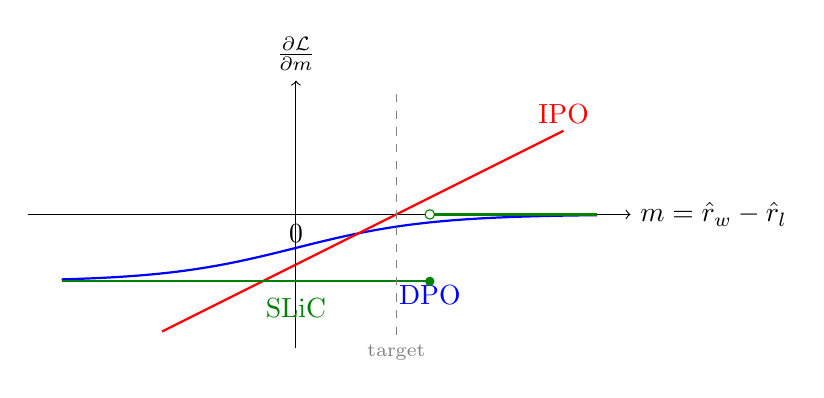
\begin{tikzpicture}[scale=0.85]
            \draw[->] (-4,0) -- (5,0) node[right] {$m = \hat{r}_w - \hat{r}_l$};
            \draw[->] (0,-2) -- (0,2) node[above] {$\frac{\partial \mathcal{L}}{\partial m}$};

            % DPO gradient: -sigmoid(-m) = -(1/(1+exp(m)))
            \draw[thick, blue, domain=-3.5:4.5, samples=100] plot (\x, {-1/(1 + exp(\x))});
            \node[blue] at (2, -1.2) {DPO};

            % IPO gradient: 2(m - target)
            \draw[thick, red, domain=-2:4, samples=50] plot (\x, {0.5*(\x - 1.5)});
            \node[red] at (4, 1.5) {IPO};

            % SLiC gradient: -1 for m < delta, 0 otherwise
            \draw[thick, green!50!black] (-3.5, -1) -- (2, -1);
            \draw[thick, green!50!black] (2, 0) -- (4.5, 0);
            \fill[green!50!black] (2, -1) circle (2pt);
            \draw[green!50!black, fill=white] (2, 0) circle (2pt);
            \node[green!50!black] at (0, -1.4) {SLiC};

            \node[below] at (0,0) {$0$};
            \draw[dashed, gray] (1.5, -1.8) -- (1.5, 1.8);
            \node[below, gray, font=\scriptsize] at (1.5, -1.8) {target};
        \end{tikzpicture}
    \end{center}

    \begin{itemize}
        \item \textbf{DPO}: Gradient $\to 0$ as $m \to \infty$, but never exactly zero. Always some signal.
        \item \textbf{IPO}: Gradient flips sign at the target. Pushes back if you overshoot.
        \item \textbf{SLiC}: Constant gradient until margin reached, then exactly zero.
    \end{itemize}
\end{remark}

\section{GRPO: Group Relative Policy Optimization}

GRPO, introduced by DeepSeek, removes the need for a critic network by using group-based advantage estimation.

\subsection{Motivation}

Standard policy gradient methods require a value function $V(s)$ to compute advantages. GRPO instead samples multiple outputs for each prompt and computes advantages relative to the group.

\begin{definition}[GRPO Objective]
    For each prompt $x$, sample a group of $G$ outputs $\{y_1, \ldots, y_G\}$ from the old policy $\pi_{\theta_{\text{old}}}$. The GRPO objective is:
    \[
        \mathcal{L}_{\text{GRPO}}(\theta) = \mathbb{E}_{x} \left[ \frac{1}{G} \sum_{i=1}^{G} \min\left( \rho_i A_i, \, \text{clip}(\rho_i, 1-\epsilon, 1+\epsilon) A_i \right) - \beta \, D_{\mathrm{KL}}(\pi_\theta \| \pi_{\text{ref}}) \right]
    \]
    where $\rho_i = \frac{\pi_\theta(y_i|x)}{\pi_{\theta_{\text{old}}}(y_i|x)}$ is the importance ratio.
\end{definition}

\begin{definition}[Group Relative Advantage]
    The advantage for output $y_i$ is computed by normalizing rewards within the group:
    \[
        A_i = \frac{r(x, y_i) - \text{mean}(\{r(x, y_j)\}_{j=1}^G)}{\text{std}(\{r(x, y_j)\}_{j=1}^G)}.
    \]
\end{definition}

\begin{remark}
    This normalization ensures zero mean and unit variance advantages within each group, providing a natural baseline without a learned critic.
\end{remark}

\subsection{Token-Level KL Penalty}

\begin{definition}[Per-Token KL]
    The KL divergence is computed at the token level:
    \[
        D_{\mathrm{KL}}(\pi_\theta \| \pi_{\text{ref}}) = \sum_{t=1}^{|y|} D_{\mathrm{KL}}\bigl(\pi_\theta(\cdot | x, y_{<t}) \,\|\, \pi_{\text{ref}}(\cdot | x, y_{<t})\bigr).
    \]
\end{definition}

\subsection{Comparison with PPO}

\begin{center}
    \begin{tabular}{lcc}
        \textbf{Aspect}      & \textbf{PPO}         & \textbf{GRPO}       \\
        \hline
        Critic network       & Required             & Not required        \\
        Advantage estimation & GAE with $V(s)$      & Group normalization \\
        Memory overhead      & High (critic params) & Lower               \\
        Samples per prompt   & Typically 1          & Multiple ($G$)      \\
    \end{tabular}
\end{center}

\section{REINFORCE Leave-One-Out (RLOO)}

RLOO is another critic-free method that uses leave-one-out baselines.

\begin{definition}[RLOO Baseline]
    For output $y_i$ in a group, the baseline is the mean reward of all other outputs:
    \[
        b_i = \frac{1}{G-1} \sum_{j \neq i} r(x, y_j).
    \]
    The advantage is simply $A_i = r(x, y_i) - b_i$.
\end{definition}

\begin{remark}
    Unlike GRPO's normalized advantages, RLOO preserves the reward scale, which may be important when reward magnitudes carry meaning.
\end{remark}

\section{KTO: Kahneman-Tversky Optimization}

KTO is designed for non-paired preference data (just labels of good/bad, not comparisons).

\begin{definition}[KTO Loss]
    \[
        \mathcal{L}_{\text{KTO}}(\theta) = \mathbb{E}_{x, y} \left[ w(y) \left( 1 - \sigma\bigl( \beta \, \text{sign}(y) \cdot (\log r_\theta(x,y) - z_{\text{ref}}) \bigr) \right) \right]
    \]
    where:
    \begin{itemize}
        \item $\log r_\theta(x,y) = \log \pi_\theta(y|x) - \log \pi_{\text{ref}}(y|x)$,
        \item $\text{sign}(y) = +1$ if $y$ is desirable, $-1$ if undesirable,
        \item $z_{\text{ref}}$ is a reference point (KL from reference on desirable examples),
        \item $w(y)$ weights desirable vs undesirable examples (often with loss aversion $\lambda > 1$ for undesirable).
    \end{itemize}
\end{definition}

\begin{remark}
    KTO is inspired by Kahneman and Tversky's prospect theory: humans are loss-averse and evaluate outcomes relative to a reference point, not absolutely.
\end{remark}

\section{Comparison of Alignment Methods}

This section provides a comprehensive comparison of all preference optimization and RL alignment methods. The goal is to make each method identifiable by its loss function structure.

\subsection{Quick Reference: Identifying Methods by Loss Function}

\begin{center}
    \renewcommand{\arraystretch}{2.2}
    \begin{tabular}{|l|l|l|}
        \hline
        \textbf{Method}                                                               & \textbf{Loss Function} & \textbf{Identifying Feature} \\
        \hline
        \textbf{PPO}                                                                  &
        $\min\bigl(r_t A_t, \text{clip}(r_t, 1{\pm}\epsilon) A_t\bigr)$               &
        Clipped ratio $\times$ advantage                                                                                                      \\
        \hline
        \textbf{DPO}                                                                  &
        $-\log \sigma\bigl(\beta(\hat{r}_w - \hat{r}_l)\bigr)$                        &
        $\sigma$ of log-ratio \emph{difference}                                                                                               \\
        \hline
        \textbf{IPO}                                                                  &
        $\bigl(\hat{r}_w - \hat{r}_l - \tfrac{1}{2\beta}\bigr)^2$                     &
        \emph{Squared} loss with margin                                                                                                       \\
        \hline
        \textbf{GRPO}                                                                 &
        $\text{PPO-clip} + \text{group-normalized } A_i$                              &
        Advantages: $\frac{r_i - \mu}{\sigma}$                                                                                                \\
        \hline
        \textbf{RLOO}                                                                 &
        REINFORCE with $b_i = \frac{1}{G-1}\sum_{j \neq i} r_j$                       &
        Leave-one-out baseline                                                                                                                \\
        \hline
        \textbf{KTO}                                                                  &
        $w(y)(1 - \sigma(\beta \cdot \text{sign}(y) \cdot \Delta))$                   &
        Uses $\text{sign}(y)$ for good/bad                                                                                                    \\
        \hline
        \textbf{SLiC-HF}                                                              &
        $\max(0, \delta - \hat{r}_w + \hat{r}_l)$                                     &
        Hinge loss (margin $\delta$)                                                                                                          \\
        \hline
        \textbf{ORPO}                                                                 &
        $\mathcal{L}_{\text{SFT}} - \lambda \log \sigma(\text{log-odds diff})$        &
        Combines SFT + odds ratio                                                                                                             \\
        \hline
        \textbf{SimPO}                                                                &
        $-\log \sigma\bigl(\frac{\beta}{|y|}(\log \pi_w - \log \pi_l) - \gamma\bigr)$ &
        Length-normalized, no $\pi_{\text{ref}}$                                                                                              \\
        \hline
    \end{tabular}
\end{center}

\noindent\textbf{Notation}: $\hat{r}_y = \beta \log \frac{\pi_\theta(y|x)}{\pi_{\text{ref}}(y|x)}$ is the implicit reward (log-ratio).

\subsection{Detailed Loss Functions}

For precise implementation, here are the complete loss functions:

\subsubsection{PPO (Proximal Policy Optimization)}
\[
    \boxed{\mathcal{L}^{\text{PPO}}(\theta) = -\mathbb{E}_t \left[ \min\left( r_t(\theta) A_t, \; \text{clip}(r_t(\theta), 1-\epsilon, 1+\epsilon) A_t \right) \right]}
\]
where $r_t(\theta) = \frac{\pi_\theta(a_t|s_t)}{\pi_{\theta_{\text{old}}}(a_t|s_t)}$ and $A_t$ is the advantage estimate (typically from GAE).

\textbf{Key identifiers}:
\begin{itemize}
    \item Ratio $r_t$ between new and \emph{old} policy (not reference!)
    \item Clipping to $[1-\epsilon, 1+\epsilon]$
    \item Requires advantage estimation (critic network or GAE)
\end{itemize}

\subsubsection{DPO (Direct Preference Optimization)}
\[
    \boxed{\mathcal{L}_{\text{DPO}}(\theta) = -\mathbb{E}_{(x, y_w, y_l)} \left[ \log \sigma\left( \beta \log \frac{\pi_\theta(y_w|x)}{\pi_{\text{ref}}(y_w|x)} - \beta \log \frac{\pi_\theta(y_l|x)}{\pi_{\text{ref}}(y_l|x)} \right) \right]}
\]

\textbf{Equivalent forms}:
\begin{align*}
     & = -\mathbb{E} \left[ \log \sigma\left( \beta \log \frac{\pi_\theta(y_w|x) \cdot \pi_{\text{ref}}(y_l|x)}{\pi_\theta(y_l|x) \cdot \pi_{\text{ref}}(y_w|x)} \right) \right] \\
     & = -\mathbb{E} \left[ \log \sigma\bigl( \hat{r}_w - \hat{r}_l \bigr) \right]
\end{align*}

\textbf{Key identifiers}:
\begin{itemize}
    \item Sigmoid of \emph{difference} of log-ratios
    \item Requires $\pi_{\text{ref}}$ (reference policy)
    \item No clipping, no advantage---pure preference loss
\end{itemize}

\subsubsection{IPO (Identity Preference Optimization)}
\[
    \boxed{\mathcal{L}_{\text{IPO}}(\theta) = \mathbb{E}_{(x, y_w, y_l)} \left[ \left( \log \frac{\pi_\theta(y_w|x)}{\pi_{\text{ref}}(y_w|x)} - \log \frac{\pi_\theta(y_l|x)}{\pi_{\text{ref}}(y_l|x)} - \frac{1}{2\beta} \right)^2 \right]}
\]

\textbf{Key identifiers}:
\begin{itemize}
    \item \textbf{Squared loss} (MSE) instead of log-sigmoid
    \item Targets a fixed margin $\frac{1}{2\beta}$ rather than pushing apart indefinitely
    \item Prevents overfitting to preference data
\end{itemize}

\subsubsection{GRPO (Group Relative Policy Optimization)}
\[
    \boxed{\mathcal{L}_{\text{GRPO}}(\theta) = -\mathbb{E}_{x} \left[ \frac{1}{G} \sum_{i=1}^{G} \min\left( \rho_i A_i, \, \text{clip}(\rho_i, 1-\epsilon, 1+\epsilon) A_i \right) \right] + \beta \, D_{\mathrm{KL}}(\pi_\theta \| \pi_{\text{ref}})}
\]
where $\rho_i = \frac{\pi_\theta(y_i|x)}{\pi_{\theta_{\text{old}}}(y_i|x)}$ and the advantage is group-normalized:
\[
    A_i = \frac{r(x, y_i) - \bar{r}}{\sigma_r}, \quad \bar{r} = \frac{1}{G}\sum_{j=1}^{G} r(x, y_j), \quad \sigma_r = \text{std}(\{r_j\}).
\]

\textbf{Key identifiers}:
\begin{itemize}
    \item PPO-style clipping
    \item \textbf{Group-normalized advantages} (z-score within batch)
    \item \textbf{No critic network}---advantage from reward normalization
    \item Explicit KL penalty (not just implicit through reference)
\end{itemize}

\subsubsection{RLOO (REINFORCE Leave-One-Out)}
\[
    \boxed{\mathcal{L}_{\text{RLOO}}(\theta) = -\mathbb{E}_x \left[ \frac{1}{G} \sum_{i=1}^{G} \log \pi_\theta(y_i|x) \cdot \left( r(x, y_i) - \frac{1}{G-1}\sum_{j \neq i} r(x, y_j) \right) \right]}
\]

\textbf{Key identifiers}:
\begin{itemize}
    \item REINFORCE gradient (no clipping)
    \item \textbf{Leave-one-out baseline}: $b_i = \frac{1}{G-1}\sum_{j \neq i} r_j$
    \item Preserves reward scale (unlike GRPO's normalization)
\end{itemize}

\subsubsection{KTO (Kahneman-Tversky Optimization)}
\[
    \boxed{\mathcal{L}_{\text{KTO}}(\theta) = \mathbb{E}_{x,y} \left[ \lambda_y \cdot \max\left(0, 1 - \sigma\bigl(\beta \cdot \text{sign}(y)(\hat{r}_y - z_0)\bigr)\right) \right]}
\]
where:
\begin{itemize}
    \item $\text{sign}(y) = +1$ for desirable, $-1$ for undesirable responses
    \item $z_0 = \mathbb{E}_{x', y' \sim \mathcal{D}_{\text{desirable}}}[\hat{r}_{y'}]$ is a reference point
    \item $\lambda_y$ implements loss aversion ($\lambda_{\text{undesirable}} > \lambda_{\text{desirable}}$)
\end{itemize}

\textbf{Key identifiers}:
\begin{itemize}
    \item Uses $\text{sign}(y)$ to handle \textbf{unpaired} good/bad data
    \item Reference point $z_0$ (prospect theory)
    \item Asymmetric weighting (loss aversion)
\end{itemize}

\subsubsection{SLiC-HF (Sequence Likelihood Calibration)}
\[
    \boxed{\mathcal{L}_{\text{SLiC}}(\theta) = \mathbb{E}_{(x, y_w, y_l)} \left[ \max\left(0, \delta - \log \frac{\pi_\theta(y_w|x)}{\pi_{\text{ref}}(y_w|x)} + \log \frac{\pi_\theta(y_l|x)}{\pi_{\text{ref}}(y_l|x)} \right) \right]}
\]

\textbf{Key identifiers}:
\begin{itemize}
    \item \textbf{Hinge loss} (max with zero)
    \item Fixed margin $\delta$ (hyperparameter)
    \item Loss is zero once margin is achieved---no further optimization
\end{itemize}

\subsubsection{ORPO (Odds Ratio Preference Optimization)}
\[
    \boxed{\mathcal{L}_{\text{ORPO}}(\theta) = \mathcal{L}_{\text{SFT}}(y_w) - \lambda \log \sigma\left( \log \frac{\text{odds}_\theta(y_w|x)}{\text{odds}_\theta(y_l|x)} \right)}
\]
where $\text{odds}_\theta(y|x) = \frac{\pi_\theta(y|x)}{1 - \pi_\theta(y|x)}$.

\textbf{Key identifiers}:
\begin{itemize}
    \item \textbf{Combines SFT loss} with preference loss
    \item Uses \textbf{odds ratio} instead of probability ratio
    \item \textbf{No reference policy} $\pi_{\text{ref}}$ needed
\end{itemize}

\subsubsection{SimPO (Simple Preference Optimization)}
\[
    \boxed{\mathcal{L}_{\text{SimPO}}(\theta) = -\mathbb{E}_{(x, y_w, y_l)} \left[ \log \sigma\left( \frac{\beta}{|y_w|} \log \pi_\theta(y_w|x) - \frac{\beta}{|y_l|} \log \pi_\theta(y_l|x) - \gamma \right) \right]}
\]

\textbf{Key identifiers}:
\begin{itemize}
    \item \textbf{No reference policy} $\pi_{\text{ref}}$
    \item \textbf{Length normalization} by $|y|$ (average log-prob per token)
    \item Target margin $\gamma$ between winner and loser
\end{itemize}

\subsection{Taxonomy: What Makes Each Method Different?}

\begin{center}
    \renewcommand{\arraystretch}{1.4}
    \begin{tabular}{l|ccccc}
        \textbf{Method} & \textbf{Needs $\pi_{\text{ref}}$} & \textbf{Needs Critic} & \textbf{Data Type} & \textbf{Online?} & \textbf{Loss Type} \\
        \hline
        PPO             & No$^*$                            & Yes                   & RL rollouts        & Yes              & Clipped surrogate  \\
        DPO             & Yes                               & No                    & Paired prefs       & No               & Log-sigmoid        \\
        IPO             & Yes                               & No                    & Paired prefs       & No               & MSE                \\
        GRPO            & Yes                               & No                    & RL rollouts        & Yes              & Clipped surrogate  \\
        RLOO            & No                                & No                    & RL rollouts        & Yes              & REINFORCE          \\
        KTO             & Yes                               & No                    & Unpaired           & No               & Prospect theory    \\
        SLiC-HF         & Yes                               & No                    & Paired prefs       & No               & Hinge              \\
        ORPO            & No                                & No                    & Paired prefs       & No               & SFT + odds         \\
        SimPO           & No                                & No                    & Paired prefs       & No               & Log-sigmoid        \\
    \end{tabular}
\end{center}

\noindent $^*$PPO in RLHF typically uses KL penalty to $\pi_{\text{ref}}$, but the core PPO algorithm doesn't require it.

\subsection{Visual Decision Tree}

\begin{center}
    \begin{tikzpicture}[
            node distance=1.5cm,
            decision/.style={diamond, draw, fill=blue!10, text width=3cm, align=center, inner sep=2pt},
            result/.style={rectangle, draw, fill=green!10, rounded corners, text width=2cm, align=center},
            arrow/.style={->, >=stealth, thick}
        ]
        % Root
        \node[decision] (q1) {Have paired preferences?};

        % Yes branch
        \node[decision, below left=1.5cm and 2cm of q1] (q2) {Want reference-free?};
        \node[result, below left=1cm and 0.5cm of q2] (orpo) {ORPO\\SimPO};
        \node[decision, below right=1cm and 0.5cm of q2] (q3) {Want margin control?};
        \node[result, below left=0.8cm and 0cm of q3] (ipo) {IPO\\SLiC};
        \node[result, below right=0.8cm and 0cm of q3] (dpo) {DPO};

        % No branch (RL-based)
        \node[decision, below right=1.5cm and 2cm of q1] (q4) {Have reward model?};
        \node[result, below left=1cm and 0.2cm of q4] (kto) {KTO};
        \node[decision, below right=1cm and 0.2cm of q4] (q5) {Want critic-free?};
        \node[result, below left=0.8cm and -0.2cm of q5] (grpo) {GRPO\\RLOO};
        \node[result, below right=0.8cm and -0.2cm of q5] (ppo) {PPO};

        % Arrows
        \draw[arrow] (q1) -- node[above left] {Yes} (q2);
        \draw[arrow] (q1) -- node[above right] {No/RL} (q4);
        \draw[arrow] (q2) -- node[left] {Yes} (orpo);
        \draw[arrow] (q2) -- node[right] {No} (q3);
        \draw[arrow] (q3) -- node[left] {Yes} (ipo);
        \draw[arrow] (q3) -- node[right] {No} (dpo);
        \draw[arrow] (q4) -- node[left] {No} (kto);
        \draw[arrow] (q4) -- node[right] {Yes} (q5);
        \draw[arrow] (q5) -- node[left] {Yes} (grpo);
        \draw[arrow] (q5) -- node[right] {No} (ppo);
    \end{tikzpicture}
\end{center}

\subsection{Gradient Comparison}

Understanding the gradients helps identify \emph{how} each method learns:

\begin{center}
    \renewcommand{\arraystretch}{1.8}
    \begin{tabular}{l|l}
        \textbf{Method} & \textbf{Gradient Structure}                                                                                                                                                              \\
        \hline
        DPO             & $\nabla_\theta \mathcal{L} \propto \underbrace{\sigma(\hat{r}_l - \hat{r}_w)}_{\text{error weight}} \bigl(\nabla \log \pi_\theta(y_w) - \nabla \log \pi_\theta(y_l)\bigr)$               \\
        IPO             & $\nabla_\theta \mathcal{L} \propto \underbrace{(\hat{r}_w - \hat{r}_l - \tfrac{1}{2\beta})}_{\text{linear error}} \bigl(\nabla \log \pi_\theta(y_w) - \nabla \log \pi_\theta(y_l)\bigr)$ \\
        PPO/GRPO        & $\nabla_\theta \mathcal{L} \propto A_t \nabla \log \pi_\theta(a_t|s_t)$ \quad (clipped when $r_t$ out of range)                                                                          \\
        SLiC-HF         & $\nabla_\theta \mathcal{L} = 0$ when margin satisfied; else like DPO                                                                                                                     \\
    \end{tabular}
\end{center}

\textbf{Key insight}: DPO's weighting $\sigma(\hat{r}_l - \hat{r}_w)$ is large when the model is ``wrong'' (assigns higher implicit reward to the loser). IPO's linear weighting is gentler and prevents over-optimization.

\subsection{When to Use What}

\begin{itemize}
    \item \textbf{DPO}: Default choice for offline preference optimization. Simple, effective, well-understood.

    \item \textbf{IPO}: When you observe DPO overfitting or want more controlled optimization.

    \item \textbf{SimPO/ORPO}: When you don't want to maintain a reference policy (simpler infrastructure).

    \item \textbf{KTO}: When you only have thumbs-up/thumbs-down data, not pairwise comparisons.

    \item \textbf{GRPO}: Online RL without the complexity of training a critic; DeepSeek's choice.

    \item \textbf{RLOO}: Similar to GRPO but preserves reward scale; simpler baseline computation.

    \item \textbf{PPO}: When you need fine-grained control, have compute for a critic, or are doing classic RL.

    \item \textbf{SLiC-HF}: When you want to stop optimizing once a margin is achieved.
\end{itemize}
